      
\documentclass{article}

\usepackage[utf8]{inputenc}
\usepackage[T1]{fontenc}
\usepackage{lmodern}
\usepackage[a4paper, textheight=680pt, textwidth=470pt]{geometry}
\usepackage{graphicx}
\usepackage[rightcaption]{sidecap}
\usepackage{caption}
\usepackage[outputdir=../]{minted}
\usepackage[italian]{babel}
\usepackage{amssymb} %per \nless 
\usepackage{amsmath}
\usepackage{hyperref}
\usepackage{url}

%  /nless è il simbolo "non minore", (< con la striscia)


\begin{document}

%\renewcommand\contentsname{Indice}

\begin{titlepage}
	\centering
	\begin{figure}
	\vspace{2.5cm}
    \centerline{
\includegraphics[height=3.2cm]{Resources/logo-uniurb-2016.jpg.eps}}
    \end{figure}
	\vspace*{\baselineskip}
	\LARGE{\bfseries Relazione relativa al progetto d'esame di Programmazione Logica e Funzionale }\\
	\Large{\ sessione estiva --- a.a. 2023/2024}\\ [0.6cm]
	\large{\textbf{\scshape{Corso di Laurea in Informatica Applicata\\ Università di Urbino}}}\\[3cm]
		{\large {\scshape Studenti:}\\[0.3cm] Barzotti Nicolas\\matricola: 313687\\
        Ramagnano Gabriele\\matricola: 315439}\\
        \vskip 1 cm
	     \large{{\scshape docente:} \\[0.3cm] Marco Bernardo}\\[1.3cm]
%\scshape fa le lettere maiuscole piccole, apprescindere di come sono scritte tra le graffe		
	
\end{titlepage}

\index 
%\newpage
\tableofcontents
%\newpage

\section{Specifica del Problema}

Scrivere un programma Haskell e un programma Prolog che, per ogni simulazione numerica da effettuare, acquisiscono da tastiera un insieme finito di parametri numerici e poi stampano su schermo il risultato del calcolo numerico. Per  simulazione numerica intendiamo la simulazione di un processo fisico mediante calcolatore, ove con simulazione di un processo fisico si fa riferimento alla rappresentazione, eventualmente approssimata, di tale processo mediante la risoluzione di equazioni e modelli matematici al calcolatore \footnote{\url{https://www.treccani.it/enciclopedia/simulazioni-di-processi-fisici-mediante-calcolatore_(Enciclopedia-della-Scienza-e-della-Tecnica)/}}. Le simulazioni numeriche coinvolte sono quattro: integrazione di equazioni differenziali di moto fugoide senza attrito, di moto fugoide con attrito, di convezione lineare a una dimensione ed di Burgers a una dimensione. 
   
\section{Analisi del Problema} 

\subsection{Dati di Ingresso del Problema}

I dati in ingresso al problema sono stati suddivisi in base all'equazione da integrare numericamente, ne segue quindi la loro descrizione.

\subsubsection*{Fugoide Senza Attrito}
Il dato in ingresso è un numero reale maggiore di zero.
Questo rappresenta il passo temporale per l'integrazione dell'equazione del moto fugoide senza attrito.
\subsubsection*{Fugoide Con Attrito}
Il dato in ingresso è un numero reale maggiore di zero. Questo rappresenta il passo temporale per l'integrazione dell'equazione del moto fugoide con attrito.
\subsubsection*{Convezione}
    I dati in ingresso per l'integrazione dell'equazione di convezione sono:
    \begin{enumerate}
        \item un numero naturale, rappresenta il numero di punti della funzione d'onda;
        \item un numero reale maggiore di zero, rappresenta la lunghezza del passo temporale.
    \end{enumerate}
\subsubsection*{Burgers}
Il dato in ingresso per l'integrazione dell'equazione di Burgers è un numero naturale. Questo rappresenta il numero di punti della funzione d'onda.

\subsection{Dati di Uscita del Problema}

\subsubsection*{Fugoide Senza Attrito}
Il dato in uscita dell'integrazione dell'equazione del moto fugoide senza attrito è una sequenza di numeri reali che rappresentano la funzione di traiettoria dell'areomobile.
\subsubsection*{Fugoide Con Attrito}
Il dato in uscita dell'integrazione dell'equazione del moto fugoide con attrito è una sequenza di numeri reali che rappresentano la funzione di traiettoria dell'areomobile.
\subsubsection*{Convezione}
Il dato in uscita dell'integrazione dell'equazione di convezione lineare a una dimensione è una sequenza di numeri reali che rappresentano i valori finali della funzione d'onda quadra.
\subsubsection*{Burgers}
Il dato in uscita all'integrazione dell'equazione di Burgers a una dimensione è una sequenza di numeri reali che rappresentano i valori finali della la funzione a dente di sega.

\subsection{Relazioni Intercorrenti tra i Dati del Problema}\label{analisi}

\subsubsection*{Fugoide Senza Attrito}
L’equazione per il moto di fugoide senza attrito è un’equazione differenziale ordinaria del secondo ordine:

\begin{equation}
z(t)'' = g - \frac{g \,z(t)}{z_t} = g \left(1 - \frac{z(t)}{z_t}\right).
\end{equation}

\noindent
Possiamo trasformare questa equazione del secondo ordine in un sistema di equazioni del primo ordine:

\begin{equation}
z'(t) = b(t)
\end{equation}

\begin{equation}
b'(t) = g\left(1-\frac{z(t)}{z_t}\right).
\end{equation}

\noindent
Un altro modo di considerare un sistema di due equazioni ordinarie del primo ordine è scrivere il sistema differenziale come un’unica equazione vettoriale:

\begin{equation}
\vec{u}  = \begin{pmatrix} z \\ b \end{pmatrix}
\end{equation}

\begin{equation}
\vec{u}'(t)  = \begin{pmatrix} b\\ g-g\frac{z(t)}{z_t} \end{pmatrix}.
\end{equation}

\noindent
La soluzione approssimativa al tempo $t_n$ è $u_n$ e la soluzione numerica dell’equazione differenziale consiste nel calcolare una sequenza di soluzioni con la seguente equazione:

\begin{equation}
u_{n+1} = u_n + \Delta t \,f(u_n) + O(\Delta t)^2.
\end{equation}

\noindent
Questa formula è chiamata metodo di Eulero. Per le equazioni di moto fugoide, il metodo di Eulero fornisce il seguente algoritmo:

\begin{align}
z_{n+1} & = z_n + \Delta t \, b_n \\
b_{n+1} & = b_n + \Delta t \left(g - \frac{g}{z_t} \, z_n \right)
\end{align}

\noindent
dove:
\begin{itemize}
\item $\Delta t$ è la lunghezza del passo temporale;
\item $g$ è la forza gravitazionale terrestre;
\item $z_n$ è l'altitudine del velivolo al passo $n$;
\item $z_t$ è l'altitudine centrale del velivolo;
\item $b_n$ è la velocità del velivolo al passo $n$.
\end{itemize}

\noindent
Il numero di passi di simulazione $n$ viene calcolato $n = \frac{T}{\Delta t}$, dove $T$ è il
tempo totale di simulazione.

\noindent 
La condizione iniziale è il valore della derivata al tempo $t=0$ ed è l'altitudine iniziale del velivolo $z_0$.

\subsubsection*{Fugoide Con Attrito}
L’equazione per il moto fugoide con attrito è un sistema di equazioni differenziali ordinarie del primo ordine: 

\begin{align}
m \frac{dv}{dt} & = - W \sin\theta - D \\
m v \, \frac{d\theta}{dt} & = - W \cos\theta + L.
\end{align}

\noindent
Per visualizzare le traiettorie di volo previste da questo modello, che dipendono sia dalla velocità di avanzamento $v$ sia dall’angolo della traiettoria $\theta$, occorre calcolare la posizione dell'aliante ad ogni istante di tempo $t$. La posizione dell’aliante su un piano verticale sarà determinata dalle coordinate $(x,y)$: 

\begin{align}
x'(t) & = v \cos(\theta) \\
y'(t) & = v \sin(\theta).
\end{align}

\noindent
L’intero sistema di equazioni discretizzate con il metodo di Eulero è:

\begin{align}
v^{n+1} & = v^n + \Delta t \left(- g\, \sin\theta^n - \frac{C_D}{C_L} \frac{g}{v_t^2} (v^n)^2 \right) \\
\theta^{n+1} & = \theta^n + \Delta t \left(- \frac{g}{v^n}\,\cos\theta^n + \frac{g}{v_t^2}\, v^n \right) \\
x^{n+1} & = x^n + \Delta t \, v^n \cos\theta^n \\
y^{n+1} & = y^n + \Delta t \, v^n \sin\theta^n.
\end{align}

\noindent
Scritto in forma vettoriale risulta: 

$$u'(t) = f(u)$$

\begin{align}
u & = \begin{pmatrix} v \\ \theta \\ x \\ y \end{pmatrix} & f(u) & = \begin{pmatrix} - g\, \sin\theta - \frac{C_D}{C_L} \frac{g}{v_t^2} v^2 \\ - \frac{g}{v}\,\cos\theta + \frac{g}{v_t^2}\, v \\ v\cos\theta \\ v\sin\theta \end{pmatrix}
\end{align}

\noindent
dove:
\begin{itemize}
\item $\Delta t$ è la lunghezza del passo temporale;
\item $g$ è la forza gravitazionale terrestre;
\item $x$ è lo spostamento orizzontale del velivolo;
\item $y$ è l'altitudine del velivolo;
\item $v$ è la velocità del velivolo;
\item $v_t$ è la velocità di trim;
\item $\theta$ è l'angolo d'inclinazione del velivolo;
\item $C_D$ è il coefficiente di resistenza dell'aria;
\item $C_L$ è il coefficiente di portanza.
\end{itemize}

\noindent
Il numero di passi di simulazione $n$ viene calcolato $n = \frac{T}{\Delta t}$, dove $T$ è il
tempo totale di simulazione.

\noindent
Le condizioni iniziali sono rappresentate dalle costanti di integrazione definite dal valore della derivata al tempo $t = 0$ :

$$
v(0) = v_0 \quad \text{and} \quad \theta(0) = \theta_0
$$
$$
x(0) = x_0 \quad \text{and} \quad y(0) = y_0.
$$

\subsubsection*{Convezione}
L’equazione di convezione lineare unidimensionale è un’equazione differenziale alle derivate parziali: 

\begin{equation}
\frac{\partial u}{\partial t} + c \frac{\partial u}{\partial x} = 0.
\end{equation}

\noindent
Per la soluzione numerica di $u(x,t)$ si sono utilizzati i pedici per denotare la posizione spaziale, come in $u_i$, e gli apici per denotare l’istante temporale, come in $u^n$ : 

$$
\begin{matrix}
& &\bullet & & \bullet & &  \bullet \\
& &u^{n+1}_{i-1} & & u^{n+1}_i & & u^{n+1}_{i+1} \\
& &\bullet & & \bullet & &  \bullet \\
& &u^n_{i-1} & & u^n_i & & u^n_{i+1} \\
& &\bullet & & \bullet & &  \bullet \\
& &u^{n-1}_{i-1} & & u^{n-1}_i & & u^{n-1}_{i+1}. \\
\end{matrix}
$$

\noindent
L’equazione per fornire la soluzione numerica del problema è data da:

\begin{equation}
u_i^{n+1} = u_i^n - c \frac{\Delta t}{\Delta x}(u_i^n-u_{i-1}^n)
\end{equation}

\noindent
dove:
\begin{itemize}
\item $\Delta t$ è la lunghezza del passo temporale;
\item $\Delta x$ è la lunghezza del passo spaziale;
\item $c$ è la velocità dell'onda.
\end{itemize}


\noindent
Le condizioni iniziali per una funzione d’onda quadra sono definite così:

\begin{equation}
u(x,0)=\begin{cases}2 & \text{dove } 0.5\leq x \leq 1,\\
1 & \text{altrimenti} 
\end{cases}
\end{equation}

\noindent
dove il dominio della soluzione numerica è definito in $x\in(0,2)$. In questo modo la lunghezza del passo spaziale viene calcolata come $\Delta x = \frac{|d|}{n - 1}$, dove $|d|$ è la distanza tra l'estremo inferiore e l'estremo superiore del dominio della soluzione numerica, $n$ il numero di punti della funzione d'onda discretizzata. Il numero totale di passi temporali $i$ è invece costante.
\noindent
Poniamo inoltre delle condizioni al contorno su $x$ in modo tale da ottenere il primo punto della funzione invariato per tutto il calcolo:

\begin{equation}
u(0,t) = c 
\end{equation}

\noindent
dove $c$ è una costante e il suo valore è pari al valore del primo punto della funzione.

\subsubsection*{Burgers}
L’equazione di Burgers unidimensionale è un’equazione differenziale alle derivate parziali: 

\begin{equation}
\frac{\partial u}{\partial t} + u \frac{\partial u}{\partial x} = \nu \frac{\partial ^2u}{\partial x^2}.
\end{equation}

\noindent
L’equazione per fornire la soluzione numerica del problema è data da: 

\begin{equation}
u_i^{n+1} = u_i^n - u_i^n \frac{\Delta t}{\Delta x} (u_i^n - u_{i-1}^n) + \nu \frac{\Delta t}{\Delta x^2}(u_{i+1}^n - 2u_i^n + u_{i-1}^n)
\end{equation}

\noindent
dove: 
\begin{itemize}
\item $\nu$ è il coefficiente di diffusione dell'onda;
\item $u$:
\begin{equation} 
- \frac{2\nu\left(-\frac{(-8t + 2x) e^{-\frac{(-4t + x)^2}{4\nu(t + 1)}}}{4\nu(t + 1)} - \frac{(-8t + 2x - 4\pi) e^{-\frac{(-4t + x - 2\pi)^2}{4\nu(t + 1)}}}{4\nu(t + 1)} \right)}{e^{-\frac{(-4t + x - 2\pi)^2}{4\nu(t + 1)}} + e^{-\frac{(-4t + x)^2}{4\nu(t + 1)}}} + 4 
\end{equation}
\end{itemize}
.


\noindent
Il passo spaziale $\Delta x$ viene calcolato come precedentemente mostrato per l'equazione di convezione. Il passo temporale $\Delta t$ viene invece calcolato come $\Delta t = \frac{\sigma\Delta x^2}{n - 1}$, dove $\sigma$ è la
costante di Courant-Friedrichs-Lewy (CFL) e $n$ il numero di punti della funzione d'onda discretizzata. Il numero di passi temporali totali è $\frac{T}{\Delta t}$, dove $T$ è il tempo totale di simulazione.

\noindent
Le condizioni iniziali sono definite:

\begin{equation}
u(x, 0).
\end{equation}

\noindent
Le condizioni al contorno sono: 

\begin{equation}
u(0) = u(2\pi).
\end{equation}


 
\section{Progettazione dell'Algoritmo}
\subsection{Scelte di Progetto}

\subsection{Passi dell'Algoritmo}
I passi dell'algoritmo per risolvere il problema sono i seguenti:

\begin{enumerate}
\item Acquisire la lunghezza del passo temporale per l'equazione di moto fugoide senza attrito: \textbf{v1.}
\item Calcolare e stampare l'integrazione numerica dell'equazione di moto fugoide senza attrito: \textbf{2.1}.
\item Acquisire la lunghezza del passo temporale per l'equazione di moto fugoide con attrito: \textbf{v1.}
\item Calcolare e stampare l'integrazione numerica dell'equazione di moto fugoide con attrito: \textbf{4.1}.
\item Acquisire il numero di punti totali della funzione d'onda per l'equazione di convezione lineare unidimensionale: \textbf{v2.} e \textbf{5.1}.
\item Calcolare e stampare l'integrazione numerica dell'equazione di convezione lineare unidimensionale: \textbf{6.1}.
\item Acquisire il numero di punti totali della funzione d'onda per l'equazione di Burgers unidimensionale: \textbf{v2.}
\item Calcolare e stampare l'integrazione numerica dell'equazione di Burgers unidimensionale: \textbf{8.1}.
\end{enumerate}

\subsubsection*{2.1 Calcolo del moto fugoide senza attrito} 
\begin{itemize}
\item Alla condizione iniziale $z_0$ si concatena il resto del calcolo numerico per l'integrazione dell'equazione:
\begin{itemize}
\item Caso base: se il numero di passi temporali è pari a zero, si effettua un passo di integrazione numerica.
\item Caso generale: se il numero di passi temporali è maggiore di zero, si effettua un passo di integrazione numerica e poi, una volta decrementato di uno il numero di passi temporali, si procede ricorsivamente sul numero di passi rimanenti. 
\end{itemize}
\end{itemize}

\subsubsection*{4.1 Calcolo del moto fugoide con attrito}
\begin{itemize}
\item Alla condizione iniziale $y_0$ si concatena il resto del calcolo numerico per l'integrazione dell'equazione:
\begin{itemize}
\item Caso base: se il numero di passi temporali è pari a zero, si effettua un passo di integrazione numerica.
\item Caso generale: se il numero di passi temporali è maggiore di zero, si effettua un passo di integrazione numerica e poi, una volta decrementato di uno il numero di passi temporali, si procede ricorsivamente sul numero di passi rimanenti. 
\end{itemize}
\end{itemize}

\subsubsection*{5.1 Acquisizione dati di convezione}
\begin{itemize}
\item Se il numero di punti è pari a zero o uno, la lunghezza del passo temporale assume come valore di default zero (oppure non viene considerata).
\item Se il numero di punti è maggiore di uno, si acquisisce la lunghezza del passo temporale: \textbf{v1.}
\end{itemize}

\subsubsection*{6.1 Calcolo dell'equazione di convezione}
\begin{itemize}
\item Se il numero di punti è zero o uno, l'integrazione numerica dell'equazione è uguale al calcolo della condizione iniziale.
\item Se il numero di punti è maggiore di uno, si calcola la condizione iniziale dell'equazione e si procede con la sua integrazione numerica: \textbf{6.2}.
\end{itemize}

\subsubsection*{6.2 Convezione: condizione iniziale e integrazione numerica temporale e spaziale}
\begin{itemize}
\item Calcolo della condizione iniziale:
\begin{itemize}
\item Si genera una lista di punti equidistanti fra loro rappresentante il dominio della funzione d'onda quadra: \textbf{a.} 
\item Si calcola su ogni punto del dominio la funzione d'onda quadra (vedi onda $u$, in \ref{analisi}, 20). 
\end{itemize}
\item Calcolo dell'integrazione numerica a partire dalla condizione iniziale:
\begin{itemize}
\item Si calcola numericamente l'integrazione della funzione rispetto al tempo:
\begin{itemize}
\item[-] Caso base: se il numero di passi temporali è uguale a zero, viene restituita la funzione d'onda quadra.
\item[-] Caso generale: se il numero di passi temporali è maggiore di zero, si decrementaa di uno il numero di passi temporali, si calcola la condizione di bordo e la si aggiunge in testa al calcolo numerico dell'integrazione della funzione rispetto allo spazio. Quest'ultima viene effettuata come segue:
\begin{itemize}
\item Caso base: se si raggiunge il numero di passi spaziali totale, si effettua un passo di integrazione numerica.
\item Caso generale: se il numero di passi spaziali complessivo non è stato ancora raggiunto, si effettua un passo di integrazione numerica e poi, una volta incrementato di uno il numero di passi spaziali, si procede ricorsivamente sul numero di passi rimanenti. 
\end{itemize}
\end{itemize}
\end{itemize}
\end{itemize}

\subsubsection*{8.1 Calcolo dell'equazione di Burgers}
\begin{itemize}
\item Se il numero di punti è zero o uno, l'integrazione numerica dell'equazione è uguale al calcolo della condizione iniziale.
\item Se il numero di punti è maggiore di uno, si calcola la condizione iniziale dell'equazione e si procede con la sua integrazione numerica: \textbf{8.2}. 
\end{itemize}

\subsubsection*{8.2 Burgers: condizione iniziale e integrazione numerica temporale e spaziale}
\begin{itemize}
\item Calcolo della condizione iniziale:
\begin{itemize}
\item Si genera una lista di punti equidistanti fra loro rappresentante il dominio della funzione d'onda a dente di sega: \textbf{a.} 
\item Si calcola su ogni punto del dominio la funzione d'onda a dente di sega (vedi onda $u$, in \ref{analisi}, 23). 
\end{itemize}
\item Calcolo dell'integrazione numerica a partire dalla condizione iniziale:
\begin{itemize}
\item Si calcola numericamente l'integrazione della funzione rispetto al tempo:
\begin{itemize}
\item[-] Caso base: se il numero di passi temporali è uguale a zero, viene restituita la funzione d'onda a dente di sega.
\item[-] Caso generale: se il numero di passi temporali è maggiore di zero, si decrementaa di uno il numero di passi temporali, si calcola la condizione di bordo e la si aggiunge in testa al calcolo numerico dell'integrazione della funzione rispetto allo spazio. Quest'ultima viene effettuata come segue:
\begin{itemize}
\item Caso base: se si raggiunge il numero di passi spaziali totale, si effettua un passo di integrazione numerica.
\item Caso generale: se il numero di passi spaziali complessivo non è stato ancora raggiunto, si effettua un passo di integrazione numerica e poi, una volta incrementato di uno il numero di passi spaziali, si procede ricorsivamente sul numero di passi rimanenti. 
\end{itemize}
\end{itemize}
\end{itemize}
\end{itemize}

\subsubsection*{a. Generazione di punti equidistanti}
\begin{itemize}
\item Se il numero di punti da generare è zero, si restituisce una lista vuota.
\item Se il numero di punti da generare è maggiore di zero, si calcola la distanza tra il bordo superiore e quello inferiore del dominio, si decrementa di uno il numero di punti totali e partendo dal bordo inferiore del dominio:
\begin{itemize}
\item Caso base: se si è raggiunto il numero massimo di punti da generare, nella lista verrà aggiunto il bordo inferiore del dominio.
\item Caso generale: se il numero massimo di punti da generare non è stato ancora raggiunto, si aggiunge il punto del bordo inferiore del dominio alla lista, si incrementa di uno il numero di punti calcolati, si calcola il punto successivo della lista sostituendolo al precedente bordo inferiore del dominio e si procede ricorsivamente sul numero di punti da generare rimasti.
\end{itemize}
\end{itemize}

\subsubsection*{v1. Validazione dell'acquisizione della lunghezza del passo temporale}
\begin{itemize}
\item Caso base: se il valore del passo temporale è maggiore di zero, allora il dato viene acquisito.
\item Caso generale: altrimenti si stampa su schermo un messaggio di errore e viene ripetuta l'acquisizione.
\end{itemize}

\subsubsection*{v2. Validazione dell'acquisizione del numero di punti di una funzione}
\begin{itemize}
\item Caso base: se il numero di punti è un intero positivo, il valore viene acquisito.
\item Caso generale: altrimenti si stampa su schermo un messaggio di errore e viene ripetuta l'acquisizione.
\end{itemize}






\section{Implementazione dell'algoritmo}

\subsection{Haskell}
\underline{File sorgente \texttt{simulazioni\_numeriche.hs}} 

\scriptsize
\begin{verbatim}
{- Programma Haskell per effettuare simulazioni numeriche -}

import Data.List {- necessario per usare: 
                    - !!,      che estrae l'n-esimo elemento di una lista;
                    - head,    che estrae il primo elemento di una lista;
                    - last,    che estrae l'ultimo elemento di una lista; 
                    - tail,    che estrae gli elementi di una lista successivi al primo;
                    - init,    che estrae gli elementi di una lista precedenti all'ultimo;
                    - abs,     che ritorna il valore assoluto di un numero;
                    - reverse, che ritorna una lista di elementi in ordine inverso;
                    - length,  che ritorna la lunghezza della lista. -}

{- Costanti globali -}

{- Estremi del dominio spaziale dell'equazione di convezione -}
inf_conv = 0.0  -- Estremo inferiore del dominio spaziale.
sup_conv = 2.0  -- Estremo superiore del dominio spaziale.

{- Forza gravitazionale terrestre. -}
c_grv :: Double
c_grv = 9.81 

{- Coefficiente di diffusione. -}
nu :: Double
nu = 0.07  

{- Velocita' di trim del velivolo, misurato in m/s. -}
v_trim :: Double
v_trim = 30.0     

{- Tipo di dato che rappresenta una coppia di elementi uguali. -}
type Coppia a = (a,a)

{-  Tipo di dato che rappresenta una quadrupla di elementi uguali. -}
type Quadrupla a = (a,a,a,a)



main :: IO()
main = do putStrLn "Progetto della sessione estiva del corso Programmazione Logica e Funzionale   "
          putStrLn "Anno 2023/2024                                                                "
          putStrLn "Corso tenuto dal prof. Marco Bernardo                                         "
          putStrLn "Progetto realizzato da: Barzotti Nicolas e Ramagnano Gabriele                 "
          
          putStrLn "--------------------------------------------------------------------"
          putStrLn "| Calcolo del moto fugoide senza attrito                           |"
          putStrLn "| Parametri iniziali:                                              |"
          putStrLn "| altitudine iniziale      = 100m,                                 |"
          putStrLn "| velocita' iniziale       = 10m/s.                                |"
          putStrLn "| Parametri di simulazione:                                        |"
          putStrLn "| secondi di simulazione   = 100s,                                 |"
          putStrLn "| costante gravitazionale  = 9.81m/(s^2).                          |"
          putStrLn "| Parametro richiesto:                                             |"
          putStrLn "| passo temporale, determina la distanza temporale                 |"
          putStrLn "| tra due punti di simulazione, un valore basso                    |"
          putStrLn "| permette una simulazione piu' accurata.                          |"
          putStrLn "| Il valore del passo temporale deve essere maggiore di zero.      |"
          putStrLn "--------------------------------------------------------------------"

          dt <- acquisisci_dato_dt
          putStrLn $ show (moto_fugoide_semplice (read dt :: Double))

          putStrLn "--------------------------------------------------------------------"
          putStrLn "| Calcolo del moto fugoide con attrito                             |"
          putStrLn "| Parametri iniziali:                                              |"
          putStrLn "| velocita' iniziale                    = velocita' di trim,       |"
          putStrLn "| angolo iniziale                       = 0rad,                    |"
          putStrLn "| spostamento laterale iniziale         = 0m,                      |"
          putStrLn "| spostamento verticale iniziale        = 1000m.                   |"
          putStrLn "| Parametri di simulazione:                                        |"
          putStrLn "| secondi di simulazione                = 100s,                    |"
          putStrLn "| velocita' di trim                     = 30m/s,                   |"
          putStrLn "| costante gravitazionale               = 9.81m/(s^2),             |"
          putStrLn "| coefficiente di resistenza dell'aria  = 0.025,                   |"
          putStrLn "| coefficiente di portanza              = 1N.                      |"
          putStrLn "| Parametro richiesto:                                             |"
          putStrLn "| passo temporale, determina la distanza temporale                 |"
          putStrLn "| tra due punti di simulazione, un valore basso                    |"
          putStrLn "| permette una simulazione piu' accurata.                          |"
          putStrLn "| Il valore del passo temporale deve essere maggiore di zero.      |"
          putStrLn "--------------------------------------------------------------------"

          dt <- acquisisci_dato_dt
          putStrLn $ show (moto_fugoide_completo (read dt :: Double))

          putStrLn "--------------------------------------------------------------------"
          putStrLn "| Calcolo del moto di convezione lineare unidimensionale di        |"
          putStrLn "| un'onda quadra                                                   |"
          putStrLn "| Parametri iniziali:                                              |"
          putStrLn "| estremo superiore del dominio spaziale          = 2.0,           |"
          putStrLn "| estremo inferiore del dominio spaziale          = 0.0,           |" 
          putStrLn "| valore della parte alta della funzione d'onda   = 2.0,           |" 
          putStrLn "| valore della parte bassa della funzione d'onda  = 1.0.           |"
          putStrLn "| Parametri di simulazione:                                        |"
          putStrLn "| numero di passi temporali da effettuare         = 25,            |" 
          putStrLn "| velocita' dell'onda                             = 1.0.           |" 
          putStrLn "| Parametri richiesti all'utente:                                  |" 
          putStrLn "| numero di punti che compongono la funzione d'onda,               |"
          putStrLn "| un valore alto permette una simulazione piu' accurata.           |"
          putStrLn "| Il valore del numero di punti dell'onda deve essere un naturale. |"
          putStrLn "| Passo temporale, determina la distanza temporale                 |"
          putStrLn "| tra due punti di simulazione, un valore basso                    |"
          putStrLn "| permette una simulazione piu' accurata.                          |"
          putStrLn "| Il valore del passo temporale deve essere maggiore di zero.      |"
          putStrLn "--------------------------------------------------------------------"

          acqui_dati_e_simul_conv

          putStrLn "--------------------------------------------------------------------"
          putStrLn "| Calcolo del moto convettivo e diffusivo unidimensionale di       |"
          putStrLn "| un'onda a dente di sega                                          |"
          putStrLn "| Parametri iniziali:                                              |"
          putStrLn "| estremo superiore del dominio spaziale  = 2.0 * pi,              |"
          putStrLn "| estremo inferiore del dominio spaziale  = 0.0.                   |" 
          putStrLn "| Parametri di simulazione:                                        |"
          putStrLn "| tempo finale di simulazione             = 0.6s,                  |" 
          putStrLn "| coefficiente di diffusione              = 1.0m^2/s,              |" 
          putStrLn "| costante di Courant-Friedrichs-Lewy     = 0.1.                   |" 
          putStrLn "| Parametri richiesti all'utente:                                  |" 
          putStrLn "| numero di punti che compongono la funzione d'onda.               |"
          putStrLn "| Il valore del numero di punti dell'onda deve essere un naturale. |"
          putStrLn "--------------------------------------------------------------------"

          nx <- acquisisci_dato_nxb 
          putStrLn $ show (moto_burgers (read nx :: Int))


{- Inizio sezione input/output -}


{- L'azione input/output acquisisci_dato_dt acquisisce un parametro numerico
   reale di simulazione, ovvero la lunghezza del passo temporale.-}

acquisisci_dato_dt :: IO String
acquisisci_dato_dt = do putStr "Digita lunghezza del passo temporale: "
                        dt <- getLine
                        if ((read dt :: Double) > 0)
                          then return dt
                        else do putStrLn "Acquisizione errata!"
                                putStrLn "Il valore deve essere maggiore di zero."
                                acquisisci_dato_dt 


{- L'azione input/output acqui_dati_e_simul_conv acquisisce due parametri numerici
   di simulazione per simulare il moto di convezione: il primo, un naturale per il 
   numero di punti della funzione d'onda; il secondo un reale per la lunghezza
   del passo temporale. In seguito all'acquisizione dei parametri calcola l'inte- 
  -grazione numerica dell'equazione di convezione. -}

acqui_dati_e_simul_conv :: IO ()
acqui_dati_e_simul_conv = do putStr "Digita il numero di punti totali della funzione d'onda: "
                             nx <- getLine
                             if (((read nx  :: Integer) == 0) ||
                                 ((read nx  :: Integer) == 1)) 
                               then putStrLn $ show (cond_iniziale (read nx :: Int) onda_quadra inf_conv sup_conv)
                             else if ((read nx :: Integer) > 1)
                               then do dt <- acquisisci_dato_dt
                                       putStrLn $ show (moto_convezione (read nx :: Int) (read dt :: Double))
                             else  do putStrLn "Acquisizione errata!"
                                      putStrLn "Il valore deve essere un numero naturale."
                                      acqui_dati_e_simul_conv


{- L'azione input/output acquisisci_dato_nxb acquisisce un parametro numerico
   naturale di simulazione, ovvero il numero totale di punti della funzione
   d'onda per il calcolo dell'equazione di Burgers. -}

acquisisci_dato_nxb :: IO String
acquisisci_dato_nxb = do putStr "Digita il numero di punti totali della funzione d'onda: "
                         nx <- getLine
                         if ((read nx :: Integer) >= 0)
                           then return nx
                         else do putStrLn "Acquisizione errata!"
                                 putStrLn "Il valore deve essere un numero naturale."
                                 acquisisci_dato_nxb 


{- Fine sezione input/output -}


{- Inizio sezione fugoide semplice -}


{- La funzione moto_fugoide_semplice simula il moto fugoide privo di attrito di un velivolo generico:
   - il suo unico argomento e' la lunghezza del passo temporale dt. -}

moto_fugoide_semplice :: Double -> [Double]
moto_fugoide_semplice dt = z0 : calc_moto_semplice (z0, b0) dt passi_temporali
   where
      z0              = 100.0               -- Altitudine iniziale del velivolo.
      b0              = 10.0                -- Velocita' iniziale del velivolo.
      tempo           = 100.0               -- Numero di secondi di simulazione.
      passi_temporali = floor(tempo/dt) + 1 -- Numero di punti in cui effettuare il calcolo.


{- La funzione calc_moto_semplice calcola numericamente l'integrazione del moto fugoide:
   - il primo argomento   e' una coppia di valori, ovvero altitudine e velocita' 
     del velivolo;
   - il secondo argomento e' la lunghezza del passo temporale dt;
   - il terzo argomento   e' il numero di passi che sono ancora da effettuare. -}

calc_moto_semplice :: Coppia Double -> Double -> Int -> [Double]
calc_moto_semplice dA@(dAA,_) dt len | len == 0  = [dBA]
                                     | otherwise = dBA : calc_moto_semplice dB dt (len - 1)
   where
      dB@(dBA,_) = passo_eulero_semplice dA dt


{- La funzione passo_eulero_semplice applica il metodo di Eulero ad una coppia di numeri.
   La funzione approssima la soluzione al tempo t_(n+1) tramite il valore della funzione 
   al tempo t_n ed un opportuno passo temporale:
   - il primo argomento   e' una coppia di valori, ovvero la posizione e direzione del 
     velivolo al momento t_n;
   - il secondo argomento e' la lunghezza del passo temporale dt. -}

passo_eulero_semplice :: Coppia Double -> Double -> Coppia Double
passo_eulero_semplice dA@(y@alt, v@vel) dt = somma_coppia dA (molt_coppia_scalare (derivata_u_semplice dA) dt)


{- La funzione derivata_u_semplice viene utilizzata per l'applicazione dell'equazione del moto fugoide:
   - il suo unico argomento e' una coppia di valori, ovvero altitudine e velocita' del velivolo. -}

derivata_u_semplice :: Coppia Double -> Coppia Double
derivata_u_semplice dA@(y@alt, v@vel) = (v, c_grv * (1-y/zt))
   where
      zt = 100.0 -- Altitudine centrale all'oscillazione.


{- Fine sezione fugoide semplice -}


{- Inizio sezione fugoide completo -}


{- La funzione moto_fugoide_completo simula il moto fugoide con attrito di un velivolo generico:
   - il suo unico argomento e' la lunghezza del passo temporale dt. -}

moto_fugoide_completo :: Double -> [[Double]]
moto_fugoide_completo dt = [x0, y0] : calc_moto_completo (v0, theta0, x0, y0) dt passi_temporali
   where
      v0              = v_trim                -- La velocita' iniziale, in questo caso quella di trim.
      theta0          = 0.0                   -- Angolo iniziale del velivolo.
      x0              = 0.0                   -- Spostamento orizzontale iniziale del velivolo.
      y0              = 1000.0                -- Altitudine iniziale del velivolo.
      tempo           = 100.0                 -- Numero di secondi di simulazione.
      passi_temporali = floor(tempo/dt) + 1   -- Numero di punti in cui effettuare il calcolo.


{- La funzione calc_moto_completo calcola numericamente l'integrazione del moto fugoide:
   - il primo argomento   e' una quadrupla di valori, ovvero velocita', angolo,
     spostamento laterale e verticale del velivolo; 
   - il secondo argomento e' la lunghezza del passo temporale dt;
   - il terzo argomento   e' il numero di passi che sono ancora da effettuare. -}

calc_moto_completo :: Quadrupla Double -> Double -> Int -> [[Double]]
calc_moto_completo dA dt len | len == 0   = [[dBC, dBD]]
                             | otherwise  = [dBC, dBD] : calc_moto_completo dB dt (len - 1)
   where
      dB@(_,_,dBC,dBD) = passo_eulero_completo dA dt


{- La funzione passo_eulero_completo applica il metodo di Eulero ad una quadrupla di numeri. 
   La funzione approssima la soluzione al tempo t_(n+1) tramite il valore della funzione 
   al tempo t_n ed un opportuno passo temporale:
   - il primo argomento   e' una quadrupla di valori, ovvero la velocita', angolo, spostamento 
     laterale e verticale del velivolo al momento t_n;
   - il secondo argomento e' la lunghezza del passo temporale dt. -}

passo_eulero_completo :: Quadrupla Double -> Double -> Quadrupla Double
passo_eulero_completo dA@(v,theta,x,y) dt = somma_quadrupla dA (molt_quadrupla_scalare (derivata_u_completo (v,theta)) dt)


{- La funzione derivata_u_completo viene utilizzata per l'applicazione dell'equazione del moto fugoide:
   - il suo unico argomento e' una coppia di valori, ovvero la velocita' e l'angolo del velivolo. -}

derivata_u_completo :: Coppia Double -> Quadrupla Double
derivata_u_completo dA@(v,theta) = (- (c_grv * sin theta) - (c_res / c_prt)*c_grv/v_trim**2*v**2,
                                    - (c_grv * cos theta / v) + c_grv/v_trim**2*v,
                                    v*cos theta,
                                    v*sin theta)
   where
      c_res = 0.025  -- Coefficiente di resistenza all'aria.
      c_prt = 1.0    -- Coefficiente di portanza.


{- Fine sezione fugoide completo -}


{- Inizio sezione funzioni ausiliarie -}


{- La funzione somma_coppia prende due coppie dello stesso tipo e 
   restituisce la coppia risultante dalla somma rispettiva degli elementi. -}

somma_coppia :: (Num a) => Coppia a -> Coppia a -> Coppia a
somma_coppia (a1,b1) (a2,b2) = (a1+a2, b1+b2)


{- La funzione molt_coppia_scalare prende una coppia di elementi numerici
   ed un valore numerico e restituisce la coppia risultante dalla 
   moltiplicazione rispettiva degli elementi:
   - il primo argomento   e' una coppia di elementi;
   - il secondo argomento e' un valore numerico.  -}

molt_coppia_scalare :: (Num a) => Coppia a -> a -> Coppia a
molt_coppia_scalare (a1,b1) b = (a1*b, b1*b)


{- La funzione somma_quadrupla prende due quadruple dello stesso tipo e 
   restituisce la quadrupla risultante dalla somma rispettiva degli elementi. -}

somma_quadrupla :: (Num a) => Quadrupla a -> Quadrupla a -> Quadrupla a
somma_quadrupla (a1,b1,c1,d1) (a2,b2,c2,d2) = (a1+a2, b1+b2, c1+c2, d1+d2)


{- La funzione molt_quadrupla_scalare prende una quadrupla di elementi numerici
   ed un valore numerico e restituisce la quadrupla risultante dalla 
   moltiplicazione rispettiva degli elementi:
   - il primo argomento   e' una quadrupla di elementi;
   - il secondo argomento e' un valore numerico. -}

molt_quadrupla_scalare :: (Num a) => Quadrupla a -> a -> Quadrupla a
molt_quadrupla_scalare (a1,b1,c1,d1) b = (a1*b, b1*b, c1*b, d1*b)


{- Fine sezione funzioni ausiliarie -}


{- Inizio sezione convezione lineare -}


{- La funzione moto_convezione simula il moto di convezione lineare unidimensionale
   della funzione d'onda quadra:
   - il primo argomento   e' il numero di punti totali della funzione d'onda;
   - il secondo argomento e' la lunghezza del passo temporale. -}

moto_convezione :: Int -> Double -> [Double]
moto_convezione nx dt = tempo_conv nt nx c dx dt (cond_iniziale nx onda_quadra inf_conv sup_conv)
   where
      nt = 25                                                       -- Numero complessivo di passi temporali.
      dx = abs(sup_conv - inf_conv) / (fromIntegral(nx :: Int) - 1) -- Distanza tra qualsiasi coppia di punti della griglia adiacenti.
      c  = 1.0                                                      -- Velocita' dell'onda.


{- La funzione tempo_conv calcola numericamente l'integrazione della
   funzione rispetto al parametro temporale dt:
   - il primo argomento   e' il numero di passi temporali totali che la
     funzione d'onda deve compiere; 
   - il secondo argomento e' il numero di passi spaziali utilizzati dal
     predicato spazio_conv;
   - il terzo argomento   e' la costante di velocita' dell'onda;     
   - il quarto argomento  e' la lunghezza del passo spaziale;
   - il quinto argomento  e' la lunghezza del passo temporale;
   - il sesto argomento   e' la funzione d'onda ricalcolata. -}

tempo_conv :: Int -> Int -> Double -> Double -> Double -> [Double] -> [Double]
tempo_conv 0 _ _ _ _ onda     = onda
tempo_conv nt nx c dx dt onda = tempo_conv (nt - 1) nx c dx dt ((head onda) : spazio_conv 1 c dx dt onda) 


{- La funzione spazio_conv calcola numericamente l'integrazione della
   funzione rispetto al parametro spaziale dx:
   - il primo argomento   e' il numero di passi temporali che la funzione
     d'onda ha compiuto;
   - il secondo argomento e' la costante di velocita' dell'onda;      
   - il terzo argomento   e' la lunghezza del passo spaziale;
   - il quarto argomento  e' la lunghezza del passo temporale;
   - il quinto argomento  e' la funzione d'onda. -}

spazio_conv :: Int -> Double -> Double -> Double -> [Double] -> [Double] 
spazio_conv i c dx dt lx  | i == length lx - 1 = [passo_eulero]
                          | otherwise          = passo_eulero : spazio_conv (i+1) c dx dt lx
   where
      passo_eulero =  lx !! i - c * dt /dx *(lx !! i - lx !! (i-1))


{- La funzione onda_quadra calcola la funzione d'onda quadra:
   - il suo unico argomento e' la lista di punti equidistanti del dominio spaziale. -}

onda_quadra :: Double -> Double
onda_quadra x | x >= 0.5 && x <= 1.0 = onda_sup
              | otherwise            = onda_inf
   where
      onda_sup = 2.0 -- Valori assunti dalla parte alta della funzione d'onda quadra.
      onda_inf = 1.0 -- Valori assunti dalla parte bassa della funzione d'onda quadra.


{- Fine sezione convezione lineare -}


{- Inizio sezione convezione-diffusione (Burgers) -}


{- La funzione moto_burgers simula il moto convettivo-diffusivo unidimensionale
   della funzione d'onda a dente di sega:
   - il suo unico argomento e' il numero di punti totali della funzione d'onda. -}

moto_burgers :: Int -> [Double]
moto_burgers nx | nx == 0 || nx == 1 = cond_iniziale nx onda_dente_sega inf sup                       
                | otherwise          = tempo_burg nt nx dx dt (cond_iniziale nx onda_dente_sega inf sup)
   where
      inf      = 0.0                                            -- Estremo inferiore del dominio spaziale. 
      sup      = 2.0 * pi                                       -- Estremo superiore del dominio spaziale. 
      dx       = abs(sup - inf) / (fromIntegral(nx :: Int) - 1) -- Distanza tra qualsiasi coppia di punti della griglia adiacenti.
      sigma    = 0.1                                            -- Costante di Courant-Friedrichs-Lewy (CFL).
      dt       = sigma * dx**2 / nu                             -- Lunghezza del passo temporale.
      t_fine   = 0.6                                            -- Tempo totale di simulazione.
      nt       = floor(t_fine / dt)                             -- Numero complessivo di passi temporali.


{- La funzione tempo_burg calcola numericamente l'integrazione della funzione rispetto al 
   parametro temporale dt:
   - il primo argomento   e' il numero di passi temporali totali che la
     funzione d'onda deve compiere; 
   - il secondo argomento e' il numero di passi spaziali utilizzati dalla
     funzione spazio_burg;       
   - il terzo argomento   e' la lunghezza del passo spaziale;
   - il quarto argomento  e' la lunghezza del passo temporale;
   - il quinto argomento  e' la funzione d'onda ricalcolata. -}

tempo_burg :: Int -> Int -> Double -> Double -> [Double] -> [Double]
tempo_burg 0 _ _ _ onda     = onda
tempo_burg nt nx dx dt onda = tempo_burg (nt - 1) nx dx dt (bordo : spazio_burg 1 dx dt onda)
   where
      bordo = head onda - head onda * dt/dx * (head onda - last onda) +
              nu*dt/dx**2 * ((head $ tail onda) - 2*(head onda) + last onda) -- Condizione di bordo.


{- La funzione spazio_burg calcola numericamente l'integrazione della
   funzione rispetto al parametro spaziale dx:
   - il primo argomento   e' l'indice per accedere agli elementi della 
     lista, viene utlizzato da passo_eulero; 
   - il secondo argomento e' la lunghezza del passo spaziale;
   - il terzo argomento   e' la lunghezza del passo temporale;
   - il quarto argomento  e' la funzione d'onda. -}

spazio_burg :: Int -> Double -> Double -> [Double] -> [Double]
spazio_burg i dx dt lx | i == length lx - 1 = [bordo]
                       | otherwise          = passo_eulero : spazio_burg (i+1) dx dt lx
   where
      bordo        = (last lx) - (last lx) * dt/dx * ((last lx) - (last $ init lx)) +
                     nu*dt/dx**2*(head lx - 2*(last lx) + (last $ init lx)) -- Condizione di bordo.
      passo_eulero = (lx !! i - lx !! i * dt/dx * (lx !! i - lx !! (i-1)) + 
                      nu*dt/dx**2*(lx !! (i+1) - 2*(lx !! i) + lx !! (i-1)))


{- La funzione onda_dente_sega calcola la funzione d'onda a dente di sega 'u':
   - il suo unico argomento e' la lista di punti equidistanti del dominio spaziale. 
   Per il calcolo dell'onda si fa uso dei predicati phi e phi_primo che sono 
   rispettivamente la funzione e la sua derivata.  -}

onda_dente_sega :: Double -> Double
onda_dente_sega x = u t0 x nu
   where
      t0 = 0.0                                                                              
      phi_primo t0 x nu = -(-8*t0 + 2*x)*exp(-(-4*t0 + x)**2/(4*nu*(t0 + 1)))/(4*nu*(t0 + 1)) - 
                          (-8*t0 + 2*x - 4*pi)*exp(-(-4*t0 + x - 2*pi)**2/(4*nu*(t0 + 1)))/(4*nu*(t0 + 1))       
      phi t0 x nu       = exp(-(x-4*t0)**2/(4*nu*(t0+1))) + exp(-(x-4*t0-2*pi)**2/(4*nu*(t0+1)))
      u t0 x nu         = -2*nu*((phi_primo t0 x nu) / (phi t0 x nu))+4


{- Fine sezione convezione-diffusione (Burgers) -}


{- Inizio sezione funzioni condivise -}


{- La funzione cond_iniziale calcola la condizione iniziale (una funzione)
   per l'integrazione numerica dell'equazione di convezione e di Burgers:
   - il primo argomento   e' il numero di punti della griglia spaziale;
   - il secondo argomento e' la funzione onda_quadra (onda_dente_sega) 
     utilizzata per il calcolo delle omonime funzioni;
   - il terzo argomento   e' l'estremo inferiore del dominio spaziale;
   - il quarto argomento  e' l'estremo superiore del dominio spaziale. -}

cond_iniziale :: Int -> (Double -> Double) -> Double -> Double -> [Double]
cond_iniziale nx onda inf sup = [onda x | x <- lx]
   where
      lx = gen_punti_equi nx inf sup


{- La funzione gen_punti_equi genera una lista di punti equidistanti tra loro:
   - il primo argomento   e' il numero di punti che si vuole generare;
   - il secondo argomento e' l'estremo inferiore della lista di punti;
   - il terzo argomento   e' l'estremo superiore della lista di punti.
   Per il calcolo dei punti si fa uso della funzione calc_punti. -}

gen_punti_equi :: Int -> Double -> Double -> [Double]
gen_punti_equi 0 _ _                  = []
gen_punti_equi nx inf sup | sup > inf = calc_punti 0 (nx - 1) inf (abs $ sup - inf) 
                          | otherwise = reverse(calc_punti 0 (nx - 1) sup (abs $ sup - inf))



calc_punti :: Int -> Int -> Double -> Double -> [Double]
calc_punti i nx inf dst | i == nx   = [inf]
                        | otherwise = inf : calc_punti (i + 1) nx (inf + (dst / fromIntegral(nx :: Int))) dst


{- Fine sezione funzioni condivise -}

\end{verbatim}

\newpage
\subsection{Prolog}
\underline{File sorgente \texttt{simulazioni\_numeriche.pro}}
\scriptsize
\begin{verbatim}
   
/* Programma Prolog per effettuare simulazioni numeriche */

main :-
    write('Progetto della sessione estiva del corso Programmazione Logica e Funzionale'), nl,
    write('Anno 2023/2024'), nl,
    write('Corso tenuto dal prof. Marco Bernardo'), nl,
    write('Progetto realizzato da: Barzotti Nicolas e Ramagnano Gabriele'), nl,

    write('--------------------------------------------------------------------'), nl,
    write('| Calcolo del moto fugoide senza attrito                           |'), nl,
    write('| Parametri iniziali:                                              |'), nl,
    write('| altitudine iniziale        = 100m,                               |'), nl,
    write('| velocita\' iniziale         = 10m/s.                              |'), nl,
    write('| Parametri di simulazione:                                        |'), nl,
    write('| secondi di simulazione     = 100s,                               |'), nl,
    write('| costante gravitazionale    = 9.81m/(s^2).                        |'), nl,
    write('| Parametro richiesto:                                             |'), nl,
    write('| passo temporale, determina la distanza temporale                 |'), nl,
    write('| tra due punti di simulazione, un valore basso                    |'), nl,
    write('| permette una simulazione piu\' accurata.                          |'), nl,
    write('| Il valore del passo temporale deve essere maggiore di zero.      |'), nl,
    write('--------------------------------------------------------------------'), nl,

    acquisisci_dato_dt(DT),                                                        
    calc_fugoide_semplice(DT, FS),
    write(FS),                                                                     nl,

    write('--------------------------------------------------------------------'), nl,
    write('| Calcolo del moto fugoide con attrito                             |'), nl,
    write('| Parametri iniziali:                                              |'), nl,
    write('| velocita\' iniziale                    = velocita\' di trim,       |'), nl,
    write('| angolo iniziale                       = 0rad,                    |'), nl,
    write('| spostamento laterale iniziale         = 0m,                      |'), nl,
    write('| spostamento verticale iniziale        = 1000m.                   |'), nl,
    write('| Parametri di simulazione:                                        |'), nl,
    write('| secondi di simulazione                = 100s,                    |'), nl,
    write('| velocita\' di trim                     = 30m/s,                   |'), nl,
    write('| costante gravitazionale               = 9.81m/(s^2),             |'), nl,
    write('| coefficiente di resistenza dell\'aria  = 0.025,                   |'), nl,
    write('| coefficiente di portanza              = 1N.                      |'), nl,
    write('| Parametro richiesto:                                             |'), nl,
    write('| passo temporale, determina la distanza temporale                 |'), nl,
    write('| tra due punti di simulazione, un valore basso                    |'), nl,
    write('| permette una simulazione piu\' accurata.                          |'), nl,
    write('| Il valore del passo temporale deve essere maggiore di zero.      |'), nl,
    write('--------------------------------------------------------------------'), nl,

    acquisisci_dato_dt(DT1),                                                       
    calc_fugoide_completo(DT1, FC),
    write(FC),                                                                     nl,

    write('--------------------------------------------------------------------'), nl,
    write('| Calcolo dell\' equazione di convezione lineare a una dimensione   |'), nl,
    write('| Parametri iniziali:                                              |'), nl,
    write('| estremo superiore del dominio spaziale   = 2.0,                  |'), nl,
    write('| estremo inferiore del dominio spaziale   = 0.0,                  |'), nl, 
    write('| valore della parte alta della funzione   = 2.0,                  |'), nl, 
    write('| valore della parte bassa della funzione  = 1.0.                  |'), nl,
    write('| Parametri di simulazione:                                        |'), nl,
    write('| numero di passi temporali da effettuare  = 25,                   |'), nl, 
    write('| velocita\' dell\'onda                      = 1.0.                  |'), nl, 
    write('| Parametri richiesti all\'utente:                                  |'), nl, 
    write('| numero di punti che compongono la funzione d\'onda,               |'), nl,
    write('| un valore alto permette una simulazione piu\' accurata.           |'), nl,
    write('| Il valore del numero di punti dell\'onda deve essere un naturale. |'), nl,
    write('| Passo temporale, determina la distanza temporale                 |'), nl,
    write('| tra due punti di simulazione, un valore basso                    |'), nl,
    write('| permette una simulazione piu\' accurata.                          |'), nl,
    write('| Il valore del passo temporale deve essere maggiore di zero.      |'), nl,
    write('--------------------------------------------------------------------'), nl,

    acquisisci_dati_conv(NXC,DT2),                                                 
    calc_convezione(NXC,DT2,CONV), 
    write(CONV),                                                                   nl,

    write('--------------------------------------------------------------------'), nl,
    write('| Calcolo dell\'equazione di Burgers a una dimensione               |'), nl,
    write('| Parametri iniziali:                                              |'), nl,
    write('| estremo superiore del dominio spaziale   = 2.0 * pi,             |'), nl,
    write('| estremo inferiore del dominio spaziale   = 0.0.                  |'), nl, 
    write('| Parametri di simulazione:                                        |'), nl,
    write('| tempo finale di simulazione              = 0.6s,                 |'), nl, 
    write('| coefficiente di diffusione               = 1.0m^2/s,             |'), nl, 
    write('| costante di Courant-Friedrichs-Lewy      = 0.1.                  |'), nl, 
    write('| Parametri richiesti all\'utente:                                  |'), nl, 
    write('| numero di punti che compongono la funzione d\'onda.               |'), nl,
    write('| Il valore del numero di punti dell\'onda deve essere un naturale. |'), nl,
    write('--------------------------------------------------------------------'), nl,

    acquisisci_dato_nxb(NXB),                                                          
    calc_burgers(NXB,BURG),
    write(BURG).


/* Inizio sezione input/output */
   

/* Il predicato acquisisci_dato_dt acquisisce un parametro numerico
   reale positivo di simulazione, ovvero la lunghezza del passo temporale. */

acquisisci_dato_dt(DT) :- write('Digita lunghezza del passo temporale: '),
                          read(DTV),
                          DTV > 0,
                          DT is DTV,
                          !;     
                          write('Acquisizione errata!'), nl,
                          write('Il valore deve essere maggiore di zero.'), nl,
                          acquisisci_dato_dt(DT).


/* Il predicato acquisisci_dati_conv acquisisce due parametri numerici
   di simulazione per l'equazione di convezione: il primo, un naturale per il 
   numero di punti della funzione d'onda; il secondo un reale positivo 
   per la lunghezza del passo temporale. */

acquisisci_dati_conv(NX,DT) :- write('Digita il numero di punti totali della funzione d\'onda: '),
                               read(NXV),
                               integer(NXV),
                               acquisisci_dato_nxc(NXV,NX,DT),
                               !;     
                               write('Acquisizione errata!'), nl,
                               write('Il valore deve essere un numero naturale.'), nl,
                               acquisisci_dati_conv(NX,DT).

acquisisci_dato_nxc(NX,NX,_)  :- (NX == 0;
                                  NX == 1).
acquisisci_dato_nxc(NX,NX,DT) :- NX > 1,
                                 acquisisci_dato_dt(DT).


/* Il predicato acquisisci_dato_nxb acquisisce un parametro numerico
   naturale di simulazione, ovvero il numero totale di punti della funzione
   d'onda per il calcolo dell'equazione di Burgers. */

acquisisci_dato_nxb(NX) :- write('Digita il numero di punti totali della funzione d\'onda: '),
                           read(NXV),
                           integer(NXV),
                           NXV >= 0,
                           NX is NXV,
                           !;     
                           write('Acquisizione errata!'), nl,
                           write('Il valore deve essere un numero naturale.'), nl,
                           acquisisci_dato_nxb(NX).

      
/* Fine sezione input/output */


/* Inizio sezione fugoide semplice */


/* Il predicato calc_fugoide_semplice calcola il moto fugoide con attrito di 
   un velivolo generico:
   - il primo argomento   e' la lunghezza del passo temporale dt;
   - il secondo argomento e' la funzione di traiettoria risultante. */

calc_fugoide_semplice(DT,[Z0|T]) :-  Z0 is 100.0,                    /* Altitudine iniziale del velivolo.             */
                                     B0 is 10.0,                     /* Angolo iniziale del velivolo.                 */
                                     PASSI is (floor(100.0/DT) + 1), /* Numero di punti in cui effettuare il calcolo. */
                                     calc_moto(Z0,B0,DT,PASSI,T).


/* Il predicato calc_moto calcola numericamente l'integrazione del moto fugoide:
   - il primo argomento   e' l'altitudine del velivolo;
   - il secondo argomento e' la velocita' del velivolo;
   - il terzo argomento   e' la lunghezza del passo temporale dt;
   - il quarto argomento  e' il numero di passi che sono ancora da effettuare;
   - il quinto argomento  e' una lista di valori numerici che rappresentano 
     l'altitudine del velivolo per ogni passo temporale. */

calc_moto(Y,V,DT,0,[YT])     :- passo_eulero(Y,V,DT,YT,_).  
calc_moto(Y,V,DT,LEN,[YT|T]) :- LEN > 0,
                                passo_eulero(Y,V,DT,YT,VT),
                                LEN1 is (LEN - 1),
                                calc_moto(YT,VT,DT,LEN1,T).


/* Il predicato passo_eulero applica il metodo di Eulero ad una coppia di numeri. Il
   predicato approssima la soluzione al tempo t_(n+1) tramite il valore del predicato 
   al tempo t_n ed un opportuno passo temporale: 
   - il primo argomento   e' l'altitudine del velivolo;
   - il secondo argomento e' la velocita' del velivolo;
   - il terzo argomento   e' la lunghezza del passo temporale dt;
   - il quarto argomento  e' l'altitudine del velivolo ricalcolata;
   - il quinto argomento  e' la velocita' del velivolo ricalcolata. */

passo_eulero(Y,V,DT,Y1,V1) :- derivata_u(Y,V,YT,VT),
                              Y1 is (Y + (YT * DT)),
                              V1 is (V + (VT * DT)).


/* Il predicato derivata_u viene utilizzato per l'applicazione dell'equazione del 
   moto fugoide:
   - il primo argomento   e' l'altitudine del velivolo;
   - il secondo argomento e' l'angolazione del velivolo;
   - il terzo argomento   e' l'altitudine del velivolo ricalcolata;
   - il quarto argomento  e' l'angolazione del velivolo ricalcolata. */

derivata_u(Y,V,V,V1) :- CG is 9.81,     /* Costante gravitazionale terrestre. */
                        ZT is 100.0,    /* Altitudine centrale all'oscillazione. */
                        V1 is CG * (1-Y/ZT).


/* Fine sezione fugoide semplice */


/* Inizio sezione fugoide completo */


/* Il predicato calc_fugoide_completo calcola il moto fugoide con attrito di 
   un velivolo generico:
   - il primo argomento   e' la lunghezza del passo temporale dt;
   - il secondo argomento e' la funzione di traiettoria risultante. */

  calc_fugoide_completo(DT,[[X0|Y0]|T]) :-  V0 is 30.0,                     /* La velocita' iniziale, in questo caso quella di trim.  */
                                            THETA0 is 0.0,                  /* Angolo iniziale del velivolo.                          */
                                            X0 is 0.0,                      /* Spostamento orizzontale iniziale del velivolo.         */
                                            Y0 is 1000.0,                   /* Altitudine iniziale del velivolo.                      */
                                            PASSI is (floor(100.0/DT) + 1), /* Numero di punti in cui effettuare il calcolo.          */
                                            calc_moto(V0,THETA0,X0,Y0,DT,PASSI,T).


/* Il predicato calc_moto calcola numericamente l'integrazione del moto fugoide:
   - il primo argomento   e' la velocita' del velivolo; 
   - il secondo argomento e' l'angolo del velivolo;
   - il terzo argomento   e' lo spostamento laterale del velivolo;
   - il quarto argomento  e' lo spostamento verticale del velivolo;
   - il quinto argomento  e' la lunghezza del passo temporale dt;
   - il sesto argomento   e' il numero di passi che sono ancora da effettuare;
   - il settimo argomento e' una lista di coppie di valori numerici che rappresentano 
     spostamento laterale e l'altitudine del velivolo per ogni passo temporale. */

calc_moto(V,THETA,X,Y,DT,0,[X1,Y1])       :- passo_eulero(V,THETA,X,Y,DT,_,_,X1,Y1).
calc_moto(V,THETA,X,Y,DT,LEN,[[X1|Y1]|T]) :- LEN > 0,
                                             passo_eulero(V,THETA,X,Y,DT,V1,THETA1,X1,Y1),
                                             LEN1 is (LEN - 1),
                                             calc_moto(V1,THETA1,X1,Y1,DT,LEN1,T).


/* Il predicato passo_eulero applica il metodo di Eulero ad una quadrupla di numeri. Il
   predicato approssima la soluzione al tempo t_(n+1) tramite il valore del predicato 
   al tempo t_n ed un opportuno passo temporale: 
   - il primo argomento   e' la velocita' del velivolo; 
   - il secondo argomento e' l'angolo del velivolo;
   - il terzo argomento   e' lo spostamento laterale del velivolo;
   - il quarto argomento  e' lo spostamento verticale del velivolo;
   - il quinto argomento  e' la lunghezza del passo temporale dt;
   - il sesto argomento   e' la velocita' del velivolo ricalcolata; 
   - il settimo argomento e' l'angolo del velivolo ricalcolato;
   - il ottavo argomento  e' lo spostamento laterale del velivolo ricalcolato;
   - il nono argomento    e' lo spostamento verticale del velivolo ricalcolato. */

passo_eulero(V,THETA,X,Y,DT,V1,THETA1,X1,Y1) :- derivata_u(V,THETA,VT,THETAT,XT,YT),
                                                V1      is (V + (VT * DT)),
                                                THETA1  is (THETA + (THETAT * DT)),
                                                X1      is (X + (XT * DT)),
                                                Y1      is (Y + (YT * DT)). 


/* Il predicato derivata_u viene utilizzato per l'applicazione dell'equazione del 
   moto fugoide:
   - il primo argomento   e' la velocita' del velivolo;
   - il secondo argomento e' l'angolazione del velivolo;
   - il terzo argomento   e' la velocita' del velivolo ricalcolata;
   - il quarto argomento  e' l'angolazione del velivolo ricalcolata;
   - il quinto argomento  e' lo spostamento laterale del velivolo ricalcolato;
   - il sesto argomento   e' lo spostamento verticale del velivolo ricalcolato. */

derivata_u(V,THETA,V1,THETA1,X1,Y1) :-  CG is 9.81,     /* Costante gravitazionale terrestre.   */
                                        CR is 0.025,    /* Coefficiente di resistenza all'aria. */
                                        CP is 1.0,      /* Coefficiente di portanza.            */
                                        VTRIM is 30.0,  /* Velocita' di trim del velivolo.      */
                                        V1 is (- (CG * sin(THETA)) - (CR / CP) * CG/VTRIM**2*V**2),
                                        THETA1 is (- (CG * cos(THETA) / V) + (CG/VTRIM**2*V)),
                                        X1 is (V * cos(THETA)),
                                        Y1 is (V * sin(THETA)).


/* Fine sezione fugoide completo */


/* Inizio sezione convezione lineare */


/* Il predicato calc_convezione calcola l'integrazione numerica
   dell'equazione di convezione lineare a una dimensione:
   - il primo argomento   e' il numero di punti totali della 
     funzione d'onda;
   - il secondo argomento e' la lunghezza del passo temporale;
   - il terzo argomento   e' l'integrazione numerica completa dell'equa-
     -zione lineare unidimensionale di convezione. */

calc_convezione(NX,_,F)  :- (NX == 0;
                             NX == 1),
                            INF is 0.0,                  /* Limite inferiore del dominio spaziale. */
                            SUP is 2.0,                  /* Limite superiore del dominio spaziale. */
                            cond_iniziale_conv(NX,INF,SUP,F).
calc_convezione(NX,DT,F) :- NX > 1,
                            NT  is 25,                   /* Numero complessivo di passi temporali
                                                            che deve effettuare l'algoritmo.       */
                            NX1 is NX - 1,
                            C   is 1.0,                  /* Velocita' dell'onda.                   */
                            INF is 0.0,                  /* Limite inferiore del dominio spaziale. */
                            SUP is 2.0,                  /* Limite superiore del dominio spaziale. */
                            DX  is abs(SUP - INF) / NX1, /* Distanza tra qualsiasi coppia di
                                                            punti della griglia adiacenti.         */
                            cond_iniziale_conv(NX,INF,SUP,ONDA),
                            tempo_conv(0,NT,NX1,C,DX,DT,ONDA,F).


/* Il predicato tempo_conv calcola numericamente l'integrazione della
   funzione rispetto al parametro temporale DT:
   - il primo argomento   e' il numero di passi temporali che la funzione
     d'onda ha compiuto;
   - il secondo argomento e' il numero di passi temporali totali che la
     funzione d'onda deve compiere; 
   - il terzo argomento   e' il numero di passi spaziali utilizzati dal
     predicato spazio_conv;
   - il quarto argomento  e' la costante di velocità dell'onda;     
   - il quinto argomento  e' la lunghezza del passo spaziale;
   - il sesto argomento   e' la lunghezza del passo temporale;
   - il settimo argomento e' la funzione d'onda ricalcolata;
   - l' ottavo argomento  e' la funzione d'onda risultante. */

tempo_conv(NT,NT,_,_,_,_,F,F).
tempo_conv(I,NT,NX1,C,DX,DT,ONDA,F) :- I < NT,
                                       I1  is I + 1,
                                       testa(ONDA,T),                
                                       spazio_conv(0,NX1,C,DX,DT,ONDA,F1), 
                                       inserisci_elem(T,F1,R),                
                                       tempo_conv(I1,NT,NX1,C,DX,DT,R,F). 


/* Il predicato spazio_conv calcola numericamente l'integrazionee della
   funzione rispetto al parametro spaziale DX:
   - il primo argomento   e' il numero di passi temporali che la funzione
     d'onda ha compiuto;
   - il secondo argomento e' il numero di passi temporali totali che la
     funzione d'onda deve compiere; 
   - il terzo argomento   e' la costante di velocità dell'onda;      
   - il quarto argomento  e' la lunghezza del passo spaziale;
   - il quinto argomento  e' la lunghezza del passo temporale;
   - il sesto argomento   e' la funzione d'onda;
   - il settimo argomento e' la funzione d'onda ricalcolata con 
     passo_eulero_conv. */

spazio_conv(NX1,NX1,_,_,_,_,[]).
spazio_conv(I,NX1,C,DX,DT,[E0|LX],[E|T]) :- I < NX1,
                                            I1 is I + 1,
                                            testa(LX,E1),
                                            passo_eulero_conv(E0,E1,C,DX,DT,EU),
                                            E  is EU,
                                            spazio_conv(I1,NX1,C,DX,DT,LX,T).


/* Il predicato passo_eulero_conv effettua il passo di Eulero:
   - il primo argomento   e' l'elemento corrente della lista;
   - il secondo argomento e' l'elemento successivo a quello corrente della lista;
   - il terzo argomento   e' la costante di velocità dell'onda;
   - il quarto argomento  e' la lunghezza del passo spaziale;
   - il quinto argomento  e' la lunghezza del passo temporale;
   - il sesto argomento   e' il valore risultante del punto applicato il passo di Eulero. */

passo_eulero_conv(E0,E1,C,DX,DT,EU) :- EU is E1 - C * (DT/DX) * (E1 - E0).


/* Il predicato cond_iniziale_conv calcola la condizione iniziale (una funzione)
   per l'integrazione numerica dell'equazione di convezione:
   - il primo argomento   e' il numero di punti della griglia spaziale;
   - il secondo argomento e' l'estremo inferiore del dominio spaziale;
   - il terzo argomento   e' l'estremo superiore del dominio spaziale; 
   - il quarto argomento  e' la funzione d'onda quadra. */

cond_iniziale_conv(NX,INF,SUP,ONDA) :- gen_punti_equi(NX,INF,SUP,L),
                                       onda_quadra(L,ONDA).


/* Il predicato onda_quadra calcola la funzione d'onda quadra:
   - il primo argomento   e' la lista di punti equidistanti del dominio
     spaziale;
   - il secondo argomento e' la funzione d'onda calcolata. */

onda_quadra([],[]).
onda_quadra([X|L1],[OSI|T]) :- X >= 0.5,
                               X =< 1.0,
                               OSI is 2.0,   /* Valori assunti dalla parte alta della
                                                funzione d'onda quadra. */
                               onda_quadra(L1,T).
onda_quadra([X|L1],[OSI|T]) :- (X < 0.5; 
                                X > 1.0),
                               OSI is 1.0,   /* Valori assunti dalla parte bassa della
                                                funzione d'onda quadra. */
                               onda_quadra(L1,T).


/* Fine sezione convezione lineare */


/* Inizio sezione equazione di Burgers */


/* Il predicato calc_burgers calcola l'integrazione numerica
   dell'equazione di Burgers a una dimensione:
   - il primo argomento e' il numero di punti totali della funzione
     d'onda;
   - il secondo argomento e' l'integrazione numerica completa dell'equa-
     -zione lineare unidimensionale di Burgers.*/

calc_burgers(NX,F) :- (NX == 0;
                       NX == 1),
                      INF is 0.0,         /* Limite inferiore del dominio spaziale. */
                      SUP is 2.0 * pi,    /* Limite superiore del dominio spaziale. */
                      cond_iniziale_burg(NX,INF,SUP,F).
calc_burgers(NX,F) :- NX1 is NX - 1,
                      T   is 0.6,                  /* Tempo totale di simulazione.                */
                      S   is 0.1,                  /* Costante di Courant-Friendrichs-Lewy (CFL). */
                      NU  is 0.07,                 /* Coefficiente di diffusione.                 */
                      INF is 0.0,                  /* Limite inferiore del dominio spaziale.      */
                      SUP is 2.0 * pi,             /* Limite superiore del dominio spaziale.      */
                      DX  is abs(SUP - INF) / NX1, /* Distanza tra qualsiasi coppia di punti
                                                      della griglia adiacenti.                    */
                      DT  is S * DX^2 / NU,        /* Lunghezza del passo temporale.              */
                      NT  is floor(T/DT),          /* Numero complessivo di passi temporali
                                                      che deve effettuare l'algoritmo.            */
                      cond_iniziale_burg(NX,INF,SUP,ONDA),
                      tempo_burg(0,NT,NX1,NU,DX,DT,ONDA,F).


/* Il predicato tempo_burg calcola numericamente l'integrazione della
   funzione rispetto al parametro temporale DT:
   - il primo argomento e' il numero di passi temporali che la funzione
     d'onda ha compiuto;
   - il secondo argomento e' il numero di passi temporali totali che la
     funzione d'onda deve compiere; 
   - il terzo argomento e' il numero di passi spaziali utilizzati dal
     predicato spazio_burg;
   - il quarto argomento e' il coefficiente di diffusione;         
   - il quinto argomento e' la lunghezza del passo spaziale;
   - il sesto argomento e' la lunghezza del passo temporale;
   - il settimo argomento e' la funzione d'onda ricalcolata;
   - l' ottavo argomento e' la funzione d'onda risultante. */

tempo_burg(NT,NT,_,_,_,_,F,F).
tempo_burg(I,NT,NX1,NU,DX,DT,ONDA,F) :- I < NT,
                                        I1  is I + 1,
                                        bordo_inf(ONDA,NU,DX,DT,BI),
                                        spazio_burg(1,NX1,NU,DX,DT,ONDA,Z),
                                        inserisci_elem(BI,Z,R),
                                        tempo_burg(I1,NT,NX1,NU,DX,DT,R,F).


/* Il predicato spazio_burg calcola numericamente l'integrazione della
   funzione rispetto al parametro spaziale DX:
   - il primo argomento   e' l'indice per accedere agli elementi della 
     lista, viene utlizzato da passo_eulero; 
   - il secondo argomento e' il numero di punti della funzione; 
   - il terzo argomento   e' il coefficiente di diffusione;  
   - il quarto argomento  e' la lunghezza del passo spaziale;
   - il quinto argomento  e' la lunghezza del passo temporale;
   - il sesto argomento   e' la funzione d'onda;
   - il settimo argomento e' la funzione d'onda ricalcolata con 
     il passo_eulero_burg e bordo_sup. */

spazio_burg(NX1,NX1,NU,DX,DT,ONDA,[F]) :- bordo_sup(ONDA,NU,DX,DT,F).
spazio_burg(I,NX1,NU,DX,DT,ONDA,[E|F]) :- I < NX1,
                                          I1 is I + 1,
                                          passo_eulero_burg(ONDA,I,NU,DX,DT,E),
                                          spazio_burg(I1,NX1,NU,DX,DT,ONDA,F).


/* Il predicato bordo_inf calcola le condizioni di bordo inferiore della funzione:
   - il primo argomento   e' la funzione d'onda;
   - il secondo argomento e' il coefficiente di diffusione;
   - il terzo argomento   e' la lunghezza del passo spaziale;
   - il quarto argomento  e' la lunghezza del passo temporale;
   - il quinto argomento  e' il valore del punto estremo inferiore della funzione.
   L'uso di last e testa consente di selezionare gli elementi in coda e in testa
   alla funzione per il calcolo della condizione. */

bordo_inf([X|LX],NU,DX,DT,BI) :- last(LX,C),
                                 testa(LX,T),
                                 BI is X - X*DT/DX * (X - C) + NU*DT/DX^2 * (T - 2*X + C).


/* Il predicato bordo_sup calcola le condizioni di bordo superiore della funzione:
   - il primo argomento   e' la funzione d'onda;
   - il secondo argomento e' il coefficiente di diffusione;
   - il terzo argomento   e' la lunghezza del passo spaziale;
   - il quarto argomento  e' la lunghezza del passo temporale;
   - il quinto argomento  e' il valore del punto estremo superiore della funzione.
   L'uso di last, testa e penultimo consente di selezionare l'ultimo, il primo e
   il penultimo elemento della funzione per il calcolo della condizione. */

bordo_sup(ONDA,NU,DX,DT,BS) :- last(ONDA,C),
                               penultimo(ONDA,P),
                               testa(ONDA,T),
                               BS is C - C*DT/DX * (C - P) + NU*DT/DX^2 * (T - 2*C + P).


/* Il predicato passo_eulero_burg effettua il passo di Eulero:
   - il primo argomento   e' la funzione d'onda;
   - il secondo argomento e' l'indice dell'elemento corrente della lista;
   - il terzo argomento   e' il coefficiente di diffusione;
   - il quarto argomento  e' la lunghezza del passo spaziale;
   - il quinto argomento  e' la lunghezza del passo temporale;
   - il sesto argomento   e' il valore risultante del punto applicato il passo di Eulero.
   L'uso del predicato nth consente di accedere agli elementi della lista tramite
   indice. Gli elementi sono indicizzati da 1 a N. */

passo_eulero_burg(ONDA,I0,NU,DX,DT,EU) :- I1 is I0 + 1,
                                          I2 is I1 + 1,
                                          nth(I0,ONDA,E0),
                                          nth(I1,ONDA,E1),
                                          nth(I2,ONDA,E2),
                                          EU is E1 - E1*DT/DX * (E1 - E0) + NU*DT/DX^2 * (E2 - 2*E1 + E0).


/* Il predicato cond_iniziale_burg calcola la condizione iniziale (una 
   funzione) per il calcolo numerico dell'equazione di Burgers:
   - il primo argomento   e' il numero di punti della griglia spaziale;
   - il secondo argomento e' l'estremo inferiore del dominio spaziale;
   - il terzo argomento   e' l'estremo superiore del dominio spaziale; 
   - il quarto argomento  e' la funzione "onda a dente di sega". */

cond_iniziale_burg(NX,INF,SUP,ONDA) :- gen_punti_equi(NX,INF,SUP,L),
                                       onda_dente_sega(L,ONDA).


/* Il predicato onda_dente_sega calcola la funzione d'onda a dente di 
   sega 'u':
   - il primo argomento   e' la lista di punti equidistanti del dominio
     spaziale;
   - il secondo argomento e' la funzione d'onda calcolata. 
   Per il calcolo dell'onda si fa uso dei predicati phi e phi_primo
   che sono rispettavamente la funzione e la sua derivata. */

onda_dente_sega([],[]).
onda_dente_sega([X|LX],[U|LU]) :- T0 is 0.0,
                                  NU is 0.07,
                                  phi_primo(X,T0,NU,F1),
                                  phi(X,T0,NU,F2),
                                  U is -2*NU*(F1 / F2)+4,
                                  onda_dente_sega(LX,LU).

phi_primo(X,T0,NU,F) :- F is -(-8*T0 + 2*X)*exp(-((-4*T0 + X)^2)/(4*NU*(T0 + 1)))/(4*NU*(T0 + 1)) - (-8*T0 +
                             2*X - 4*pi)*exp(-((-4*T0 + X - 2*pi)^2)/(4*NU*(T0 + 1)))/(4*NU*(T0 + 1)).

phi(X,T0,NU,F) :- F is exp(-((X-4*T0)^2)/(4*NU*(T0+1))) + exp(-((X-4*T0-2*pi)^2)/(4*NU*(T0+1))).


/* Fine sezione equazione di Burgers */


/* Inizio sezione funzioni condivise */


/* Il predicato gen_punti_equi genera una lista di punti equidistanti tra loro:
   - il primo argomento   e' il numero di punti che si vuole generare;
   - il secondo argomento e' l'estremo inferiore della lista di punti;
   - il terzo argomento   e' l'estremo superiore della lista di punti;
   - il quarto argomento  e' la lista di punti equidistanti. 
   Per il calcolo dei punti si fa uso del predicato calc_punti. */

gen_punti_equi(0,_,_,[]).
gen_punti_equi(N,INF,SUP,L) :- N > 0,
                               DST is abs(SUP - INF),
                               N1  is N - 1, 
			                      ((SUP > INF,
                                calc_punti(0,N1,INF,DST,L));
                                (calc_punti(0,N1,SUP,DST,L1),
                                reverse(L1,L))).


calc_punti(N1,N1,INF,_,[INF]).
calc_punti(I,N1,INF,DST,[INF|L]) :- I < N1,
                                    I1   is I + 1,
                                    INF1 is INF + (DST/N1),
                                    calc_punti(I1,N1,INF1,DST,L).

/* Predicato che inserisce un elemento in testa alla lista. */

inserisci_elem(X,L,[X|L]).


/* Predicato che estrae la lista di elementi successivi al primo. */

estrai_lista([_|LX],LX).


/* Predicato per estrarre il primo elemento di una lista. */

testa([X|_],X).


/* Predicato che restituisce il penultimo elemento di una lista. */

penultimo(LX,X) :- reverse(LX,LXInv),
                   estrai_lista(LXInv,Y),
                   testa(Y,X).


/* Predicato per aggiungere un elemento alla fine di una lista. */

accoda_elem(X,[],[X]).
accoda_elem(X,[Y|L],[Y|LX]) :- accoda_elem(X,L,LX).


/* Fine sezione funzioni condivise */

\end{verbatim}


\section{Testing}

\subsection{Haskell}

\subsubsection*{Test 1}
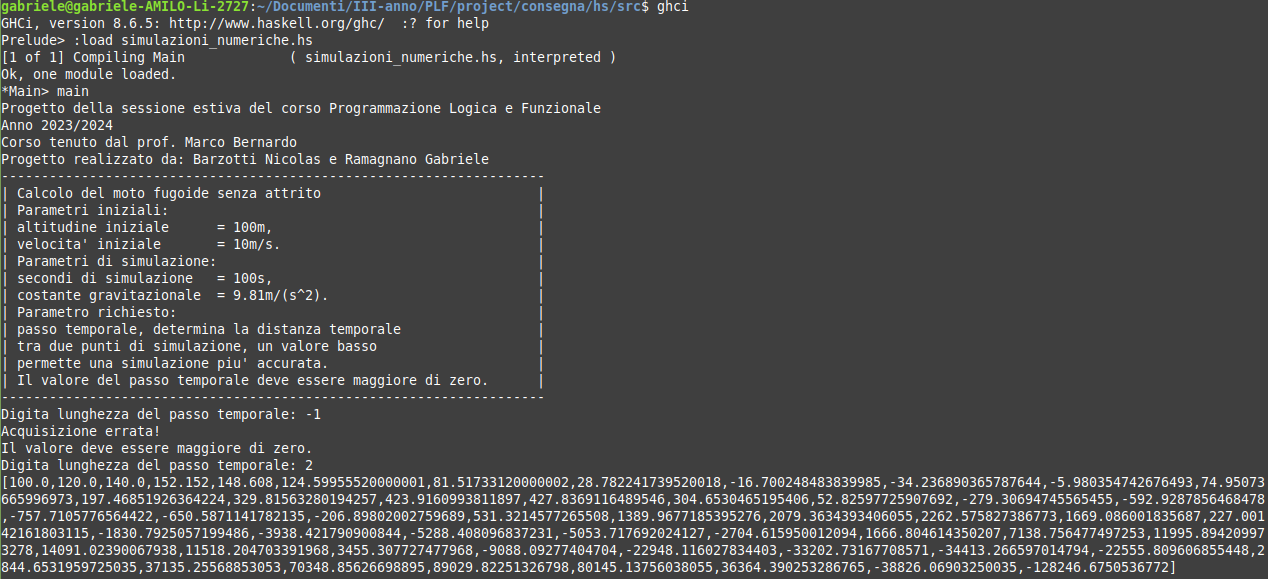
\includegraphics[width=\textwidth,height=\textheight,keepaspectratio]{05_testing/image/hs/01_test/01_negativo.png}
\\
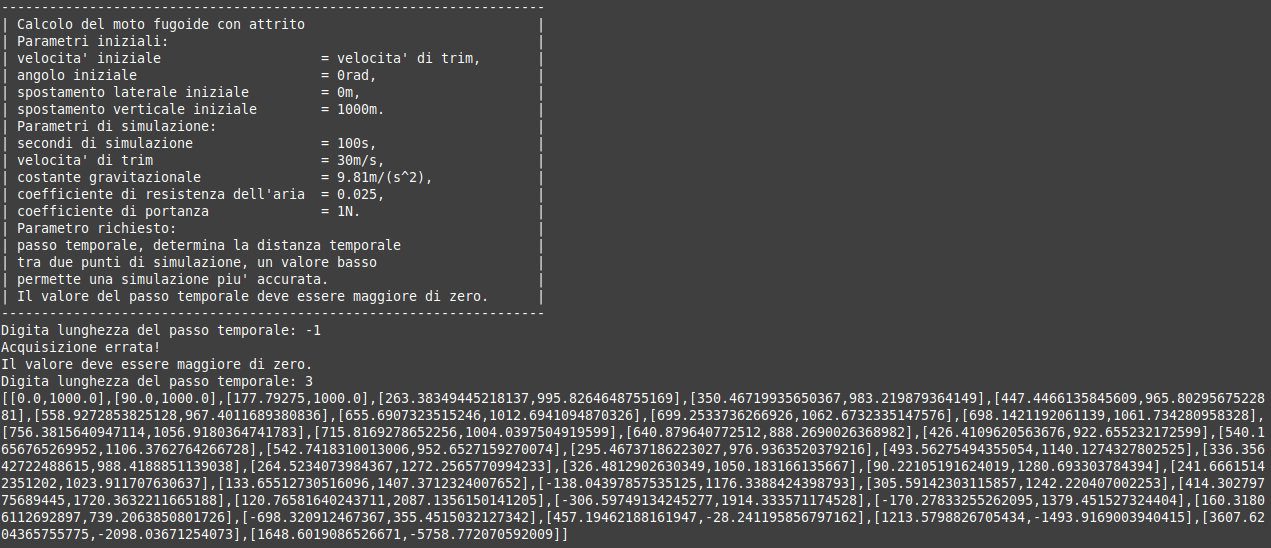
\includegraphics[width=\textwidth,height=\textheight,keepaspectratio]{05_testing/image/hs/01_test/02_negativo.png}
\\
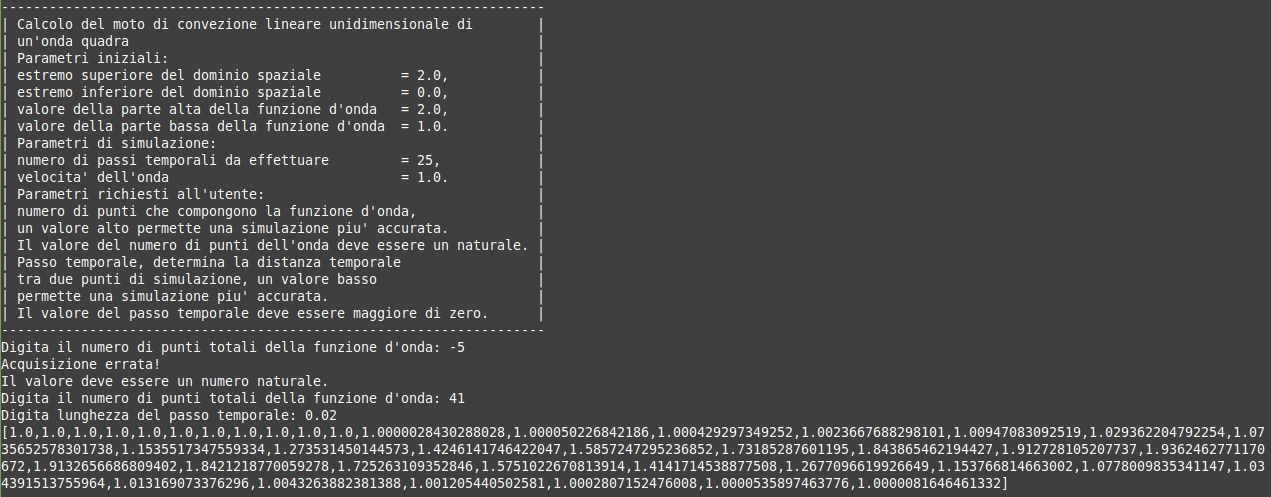
\includegraphics[width=\textwidth,height=\textheight,keepaspectratio]{05_testing/image/hs/01_test/03_negativo.png}
\\
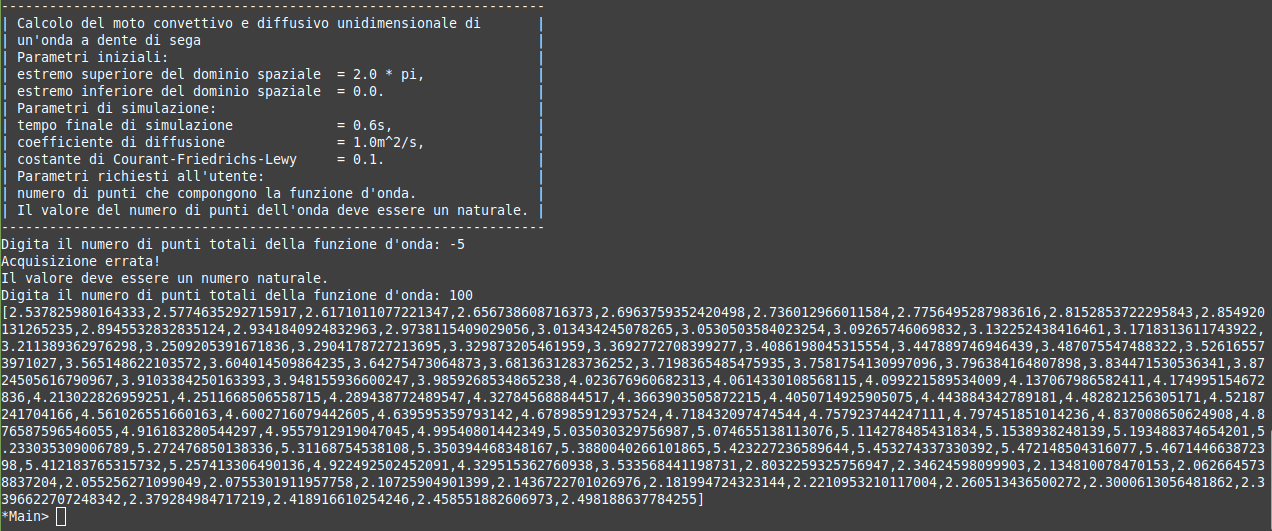
\includegraphics[width=\textwidth,height=\textheight,keepaspectratio]{05_testing/image/hs/01_test/04_negativo.png}

\subsubsection*{Test 2}
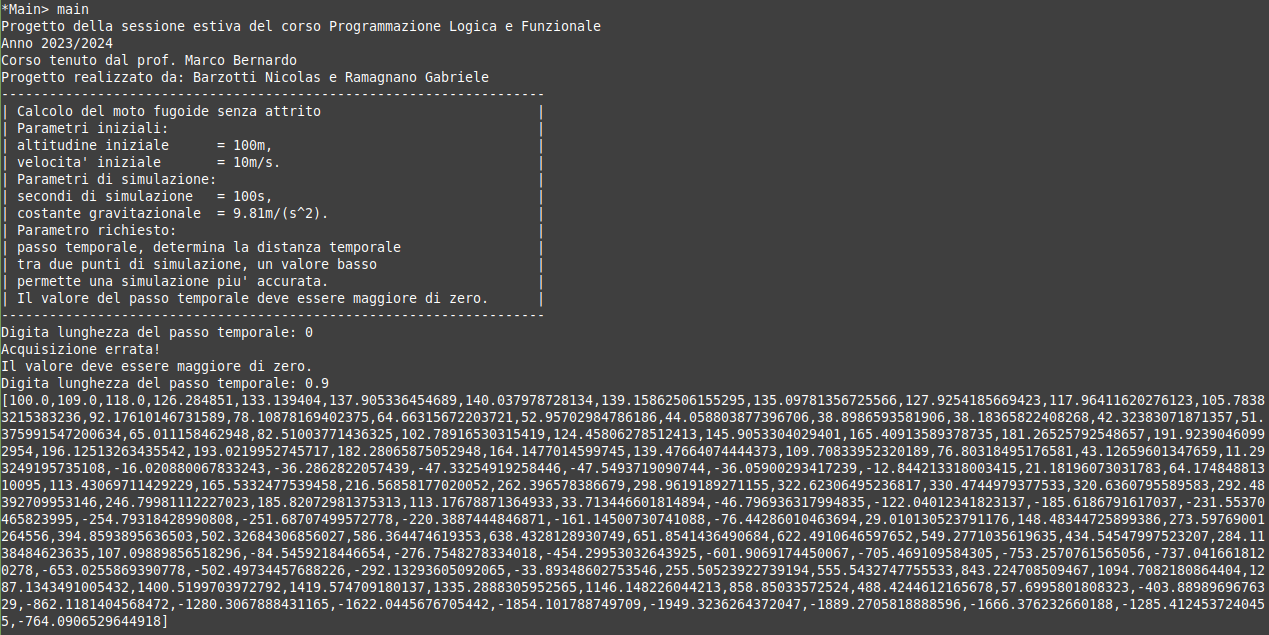
\includegraphics[width=\textwidth,height=\textheight,keepaspectratio]{05_testing/image/hs/02_test/01_zero.png}
\\
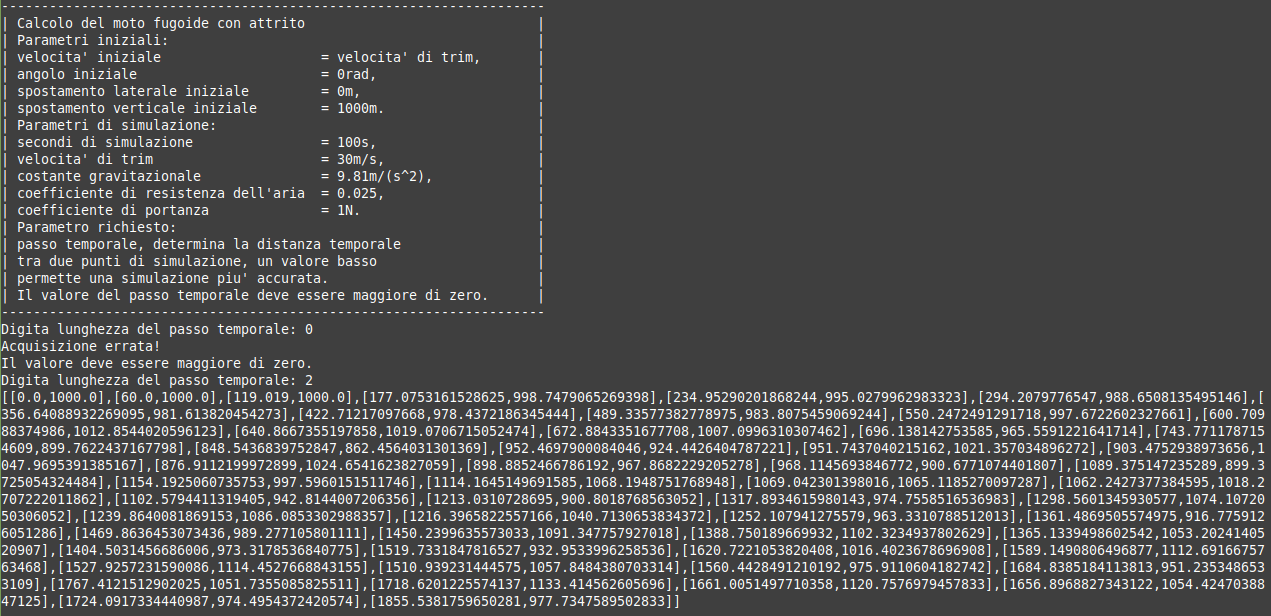
\includegraphics[width=\textwidth,height=\textheight,keepaspectratio]{05_testing/image/hs/02_test/02_zero.png}
\\
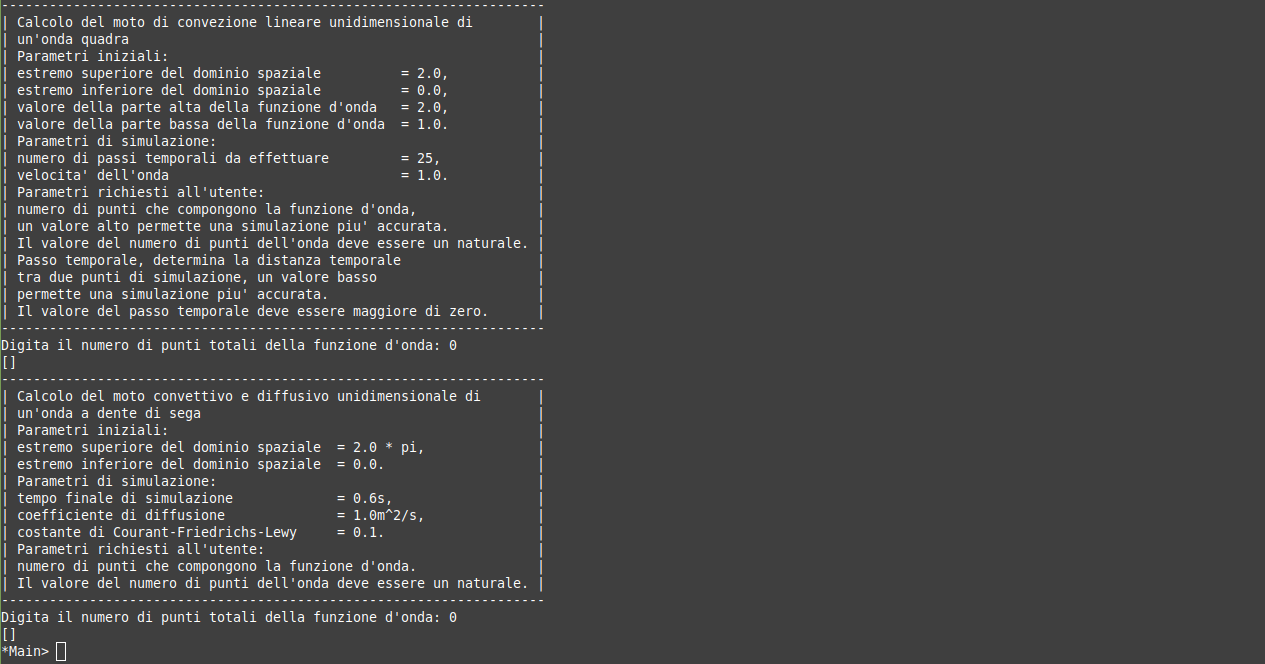
\includegraphics[width=\textwidth,height=\textheight,keepaspectratio]{05_testing/image/hs/02_test/03_zero.png}


\subsubsection*{Test 3}
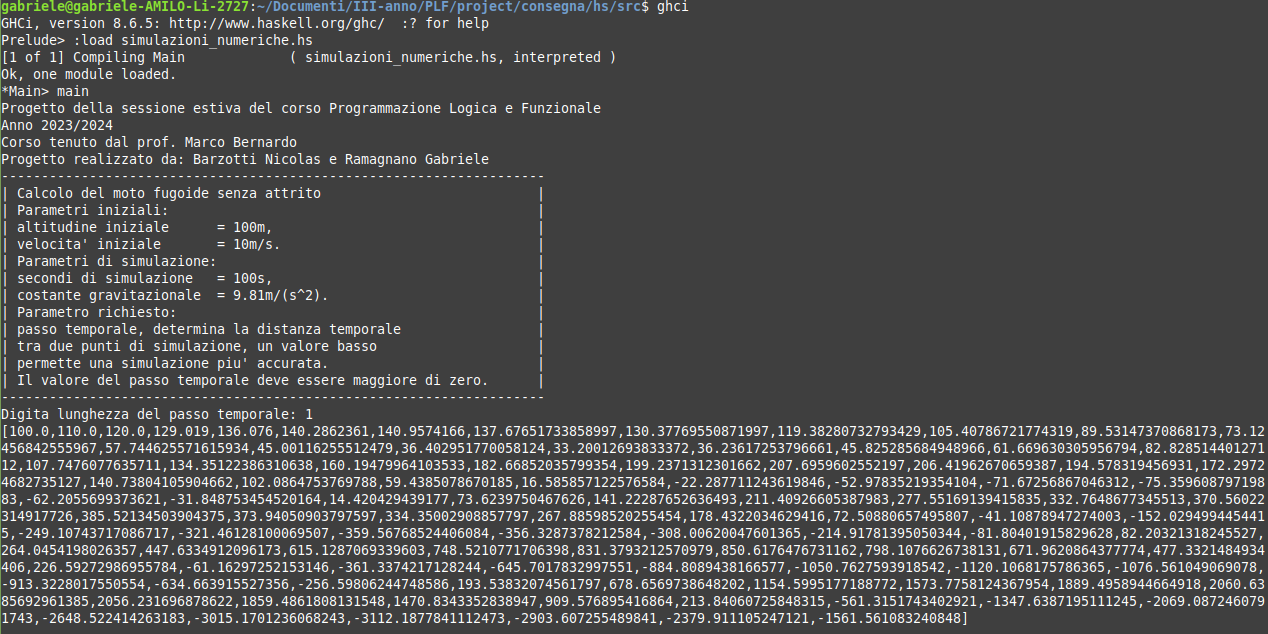
\includegraphics[width=\textwidth,height=\textheight,keepaspectratio]{05_testing/image/hs/03_test/01_uno.png}
\\
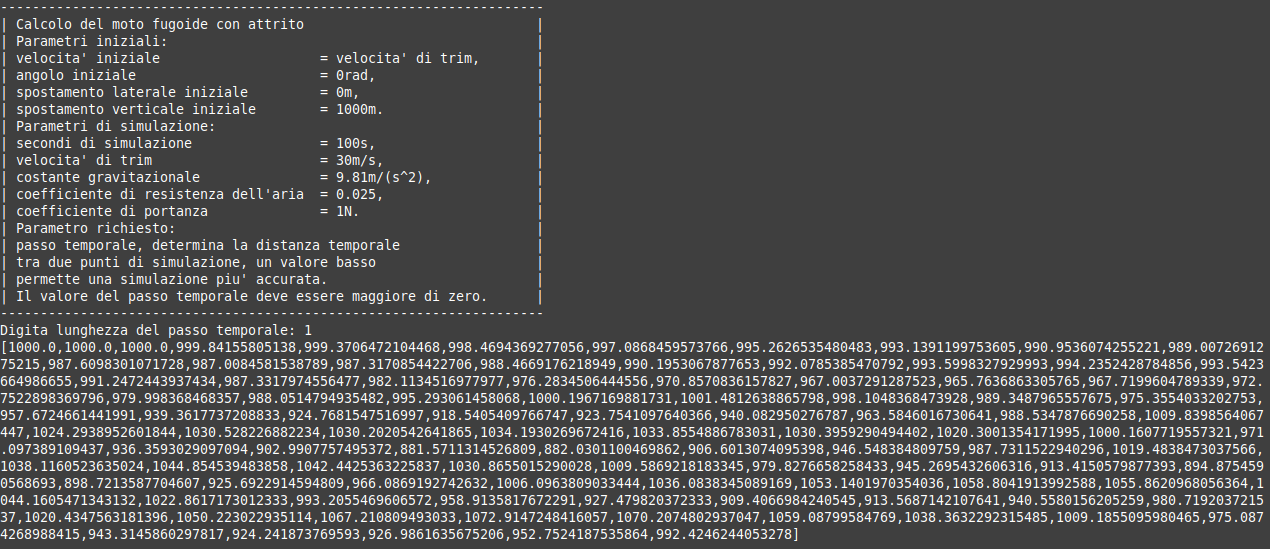
\includegraphics[width=\textwidth,height=\textheight,keepaspectratio]{05_testing/image/hs/03_test/02_uno.png}
\\
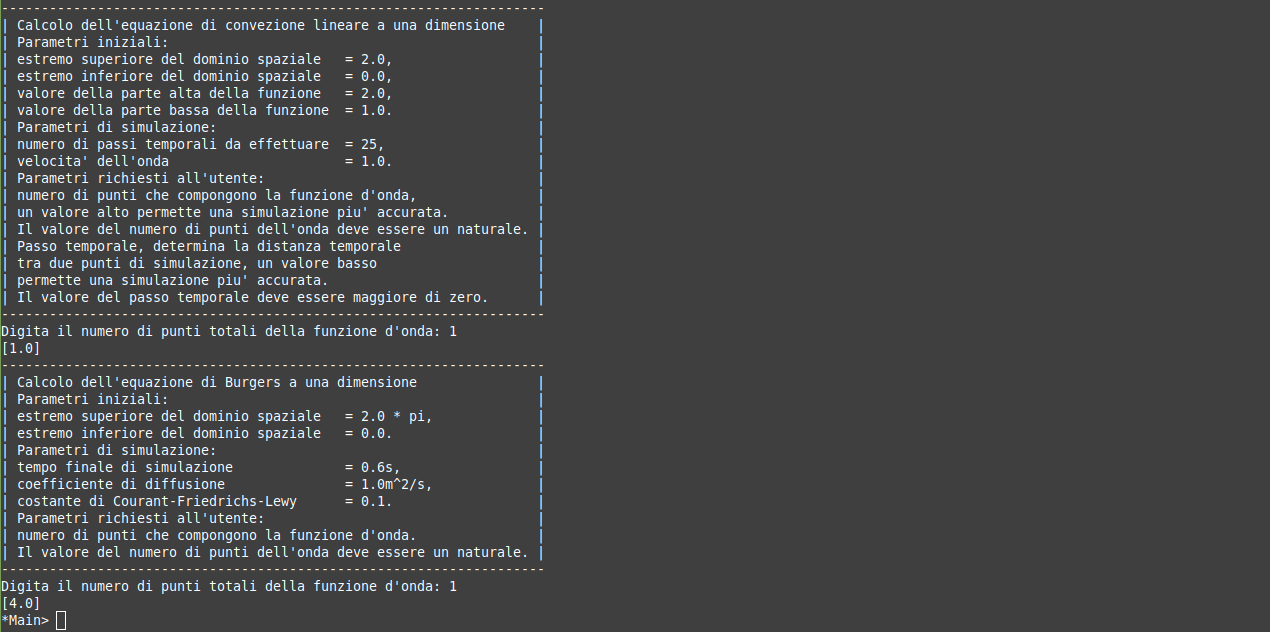
\includegraphics[width=\textwidth,height=\textheight,keepaspectratio]{05_testing/image/hs/03_test/03_uno.png}

\subsubsection*{Test 4}
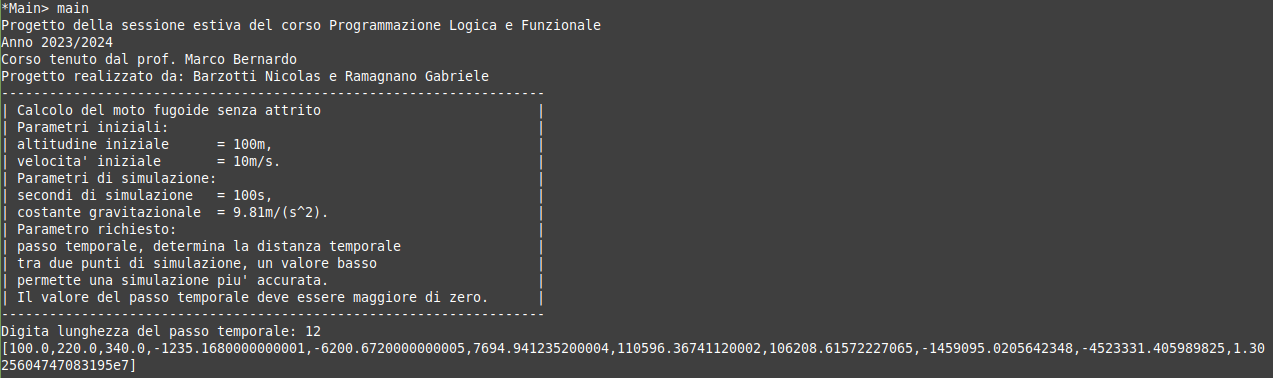
\includegraphics[width=\textwidth,height=\textheight,keepaspectratio]{05_testing/image/hs/04_test/01_normale.png}
\\
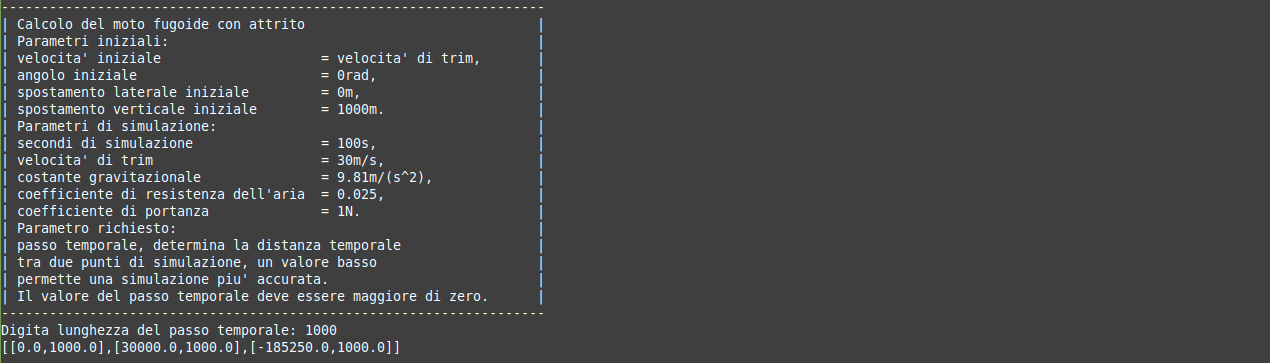
\includegraphics[width=\textwidth,height=\textheight,keepaspectratio]{05_testing/image/hs/04_test/02_normale.png}
\\
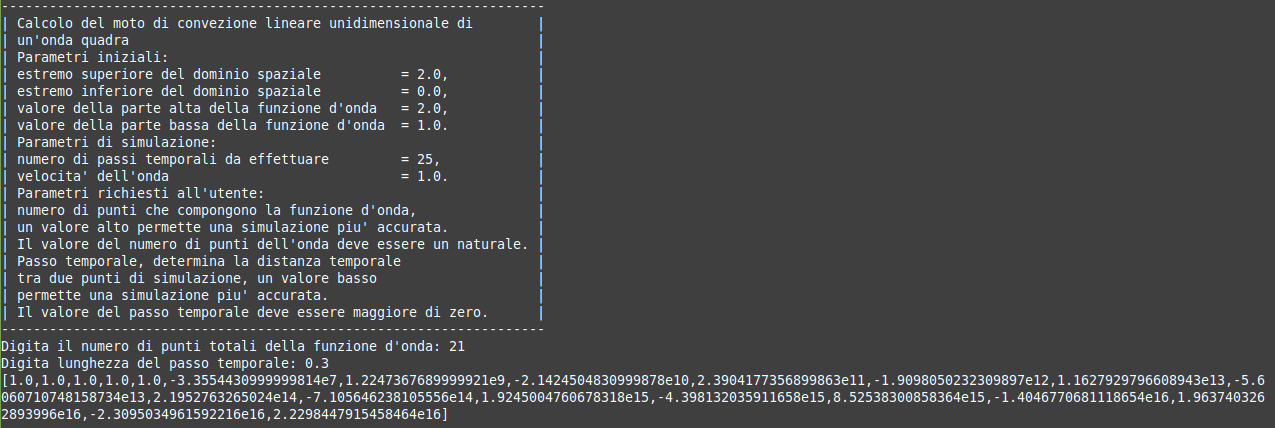
\includegraphics[width=\textwidth,height=\textheight,keepaspectratio]{05_testing/image/hs/04_test/03_normale.png}
\\
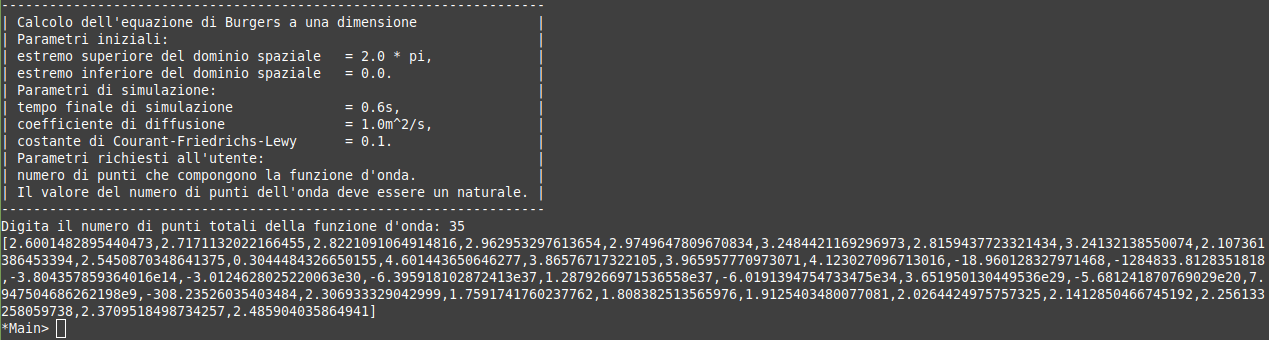
\includegraphics[width=\textwidth,height=\textheight,keepaspectratio]{05_testing/image/hs/04_test/04_normale.png}

\subsubsection*{Test 5}
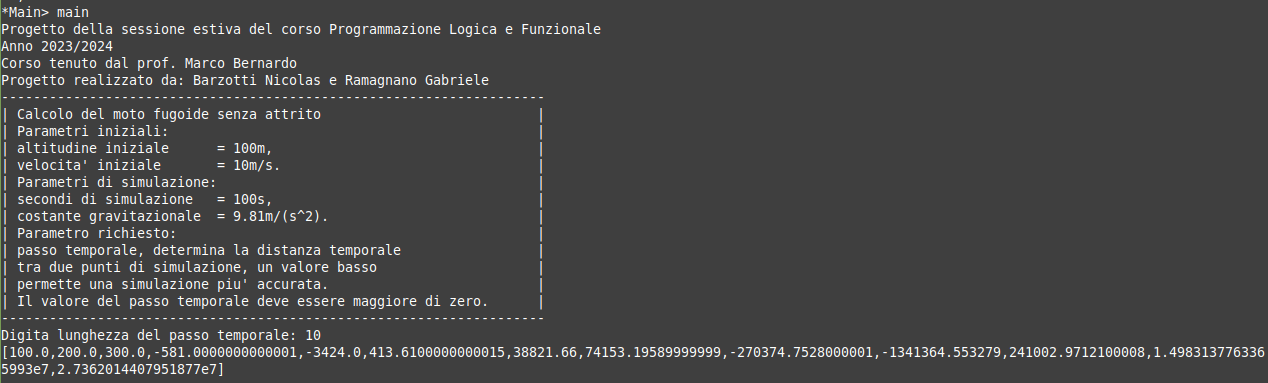
\includegraphics[width=\textwidth,height=\textheight,keepaspectratio]{05_testing/image/hs/05_test/01_misto.png}
\\
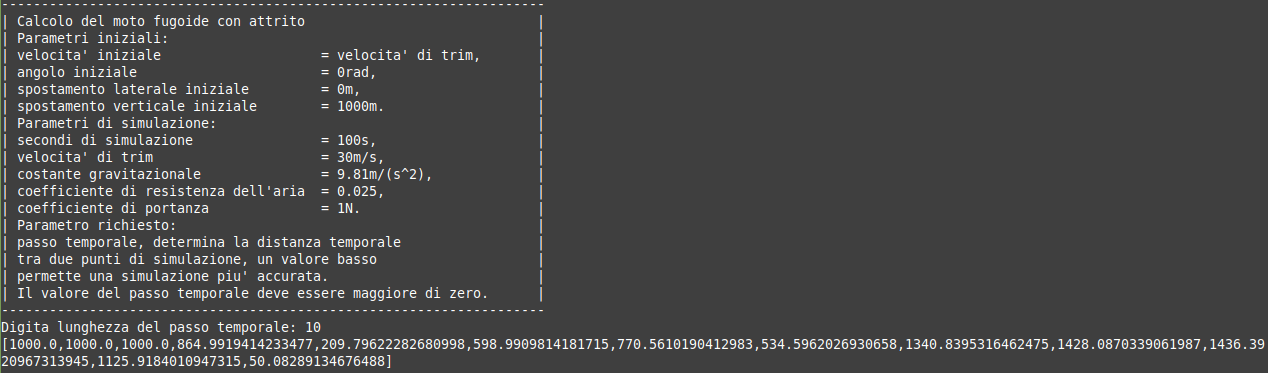
\includegraphics[width=\textwidth,height=\textheight,keepaspectratio]{05_testing/image/hs/05_test/02_misto.png}
\\
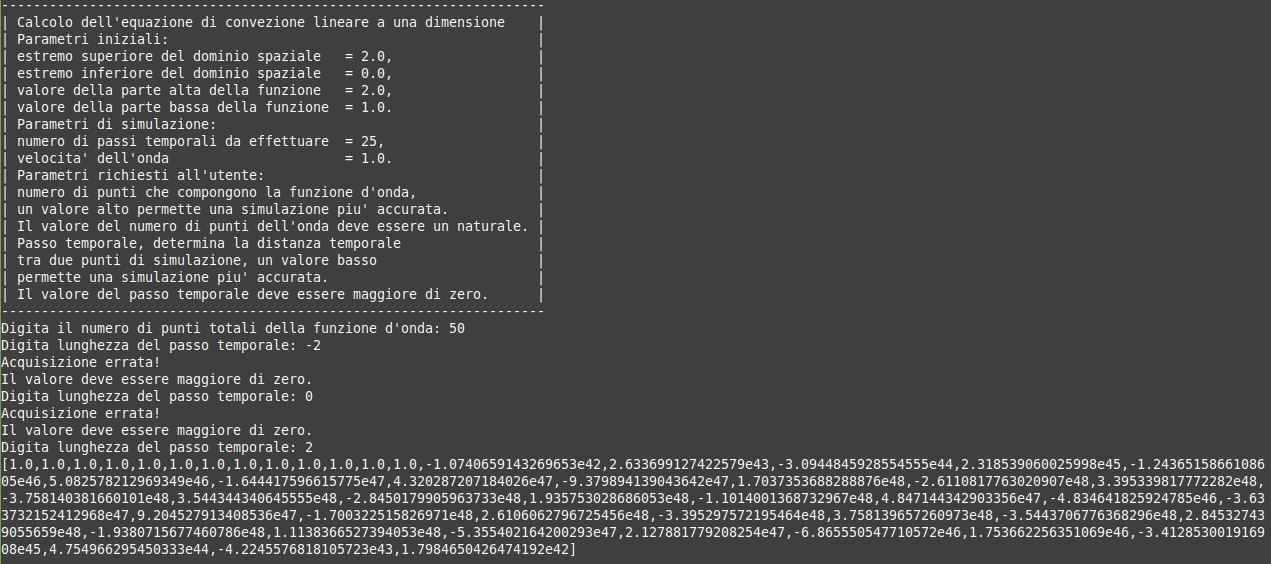
\includegraphics[width=\textwidth,height=\textheight,keepaspectratio]{05_testing/image/hs/05_test/03_misto.png}
\\
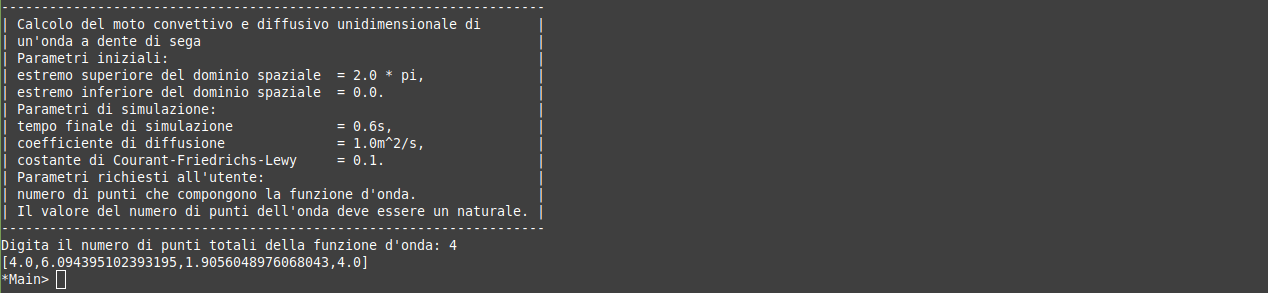
\includegraphics[width=\textwidth,height=\textheight,keepaspectratio]{05_testing/image/hs/05_test/04_misto.png}

\subsubsection*{Test 6}
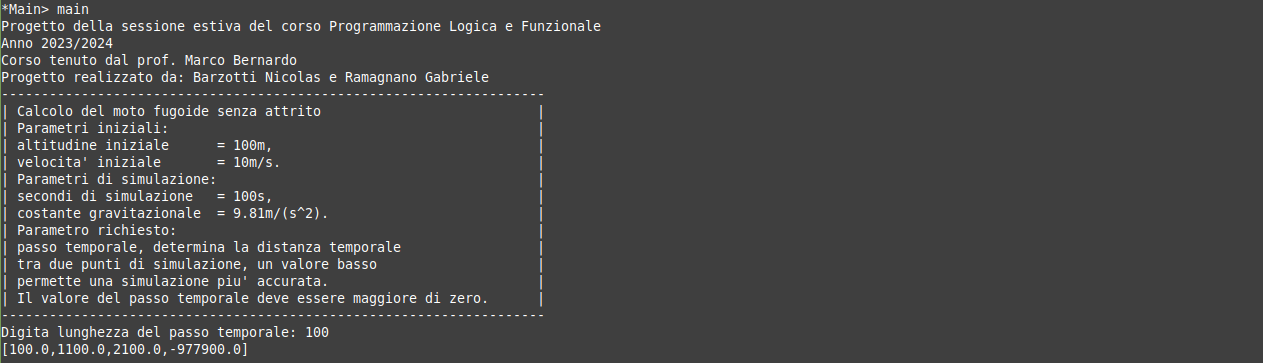
\includegraphics[width=\textwidth,height=\textheight,keepaspectratio]{05_testing/image/hs/06_test/01_misto.png}
\\
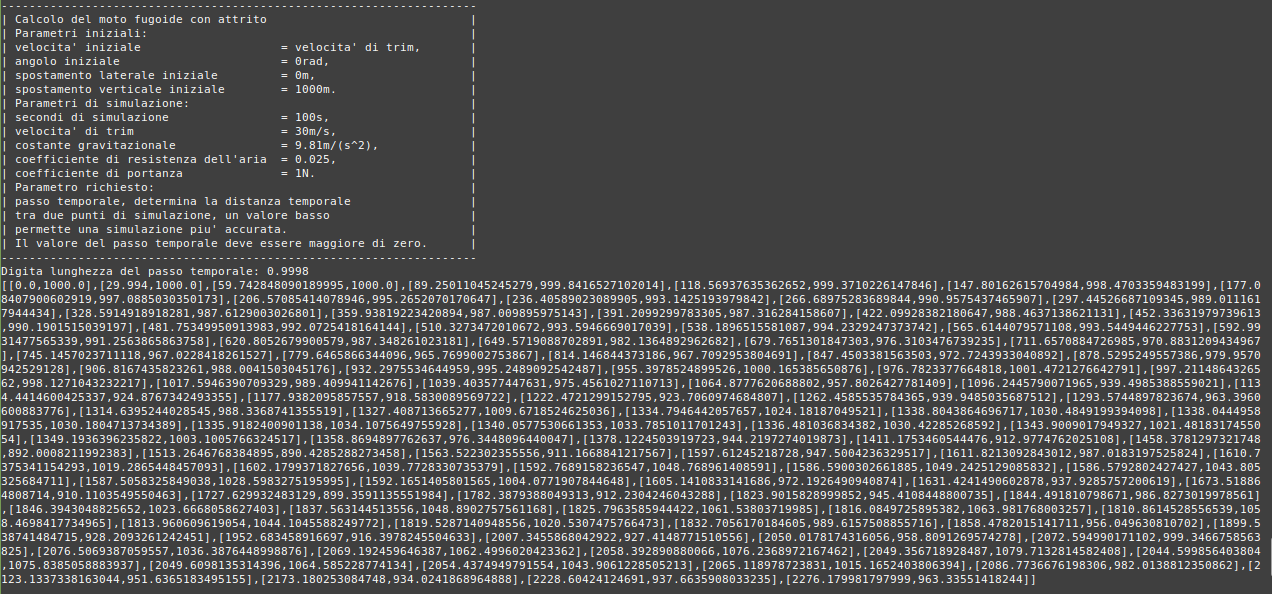
\includegraphics[width=\textwidth,height=\textheight,keepaspectratio]{05_testing/image/hs/06_test/02_misto.png}
\\
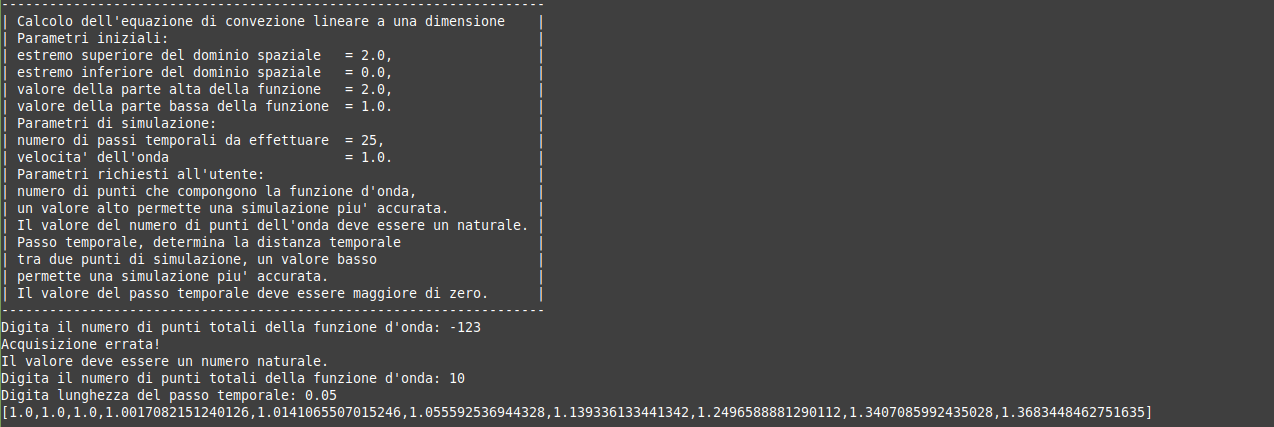
\includegraphics[width=\textwidth,height=\textheight,keepaspectratio]{05_testing/image/hs/06_test/03_misto.png}
\\
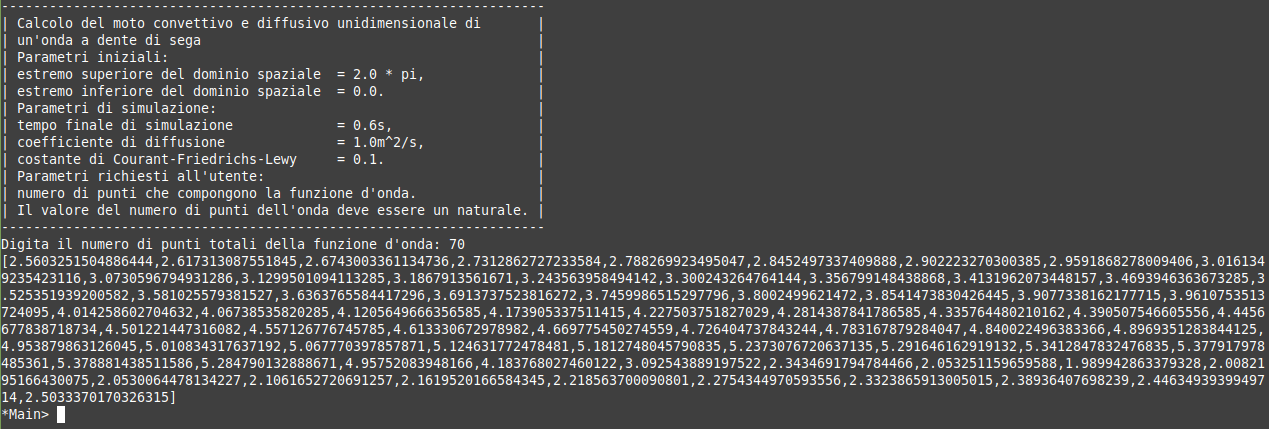
\includegraphics[width=\textwidth,height=\textheight,keepaspectratio]{05_testing/image/hs/06_test/04_misto.png}

\subsubsection*{Test 7}
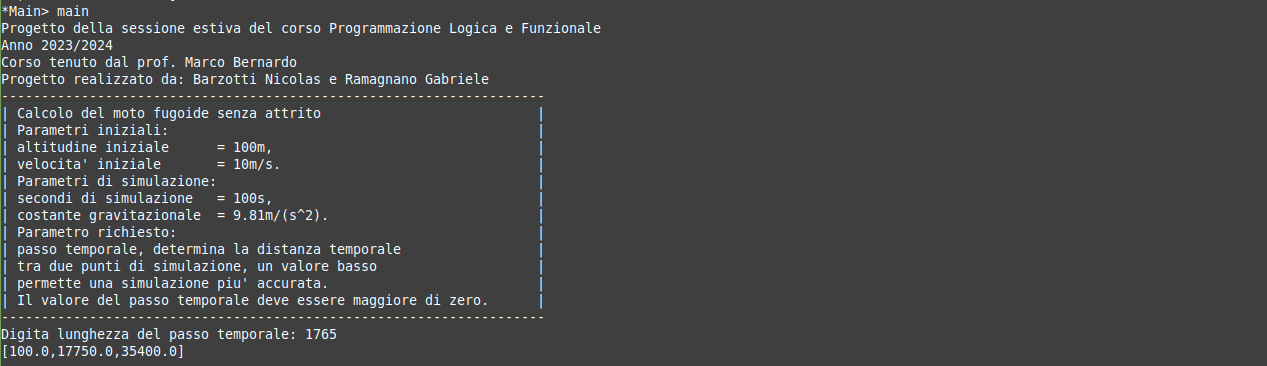
\includegraphics[width=\textwidth,height=\textheight,keepaspectratio]{05_testing/image/hs/07_test/01_misto.png}
\\
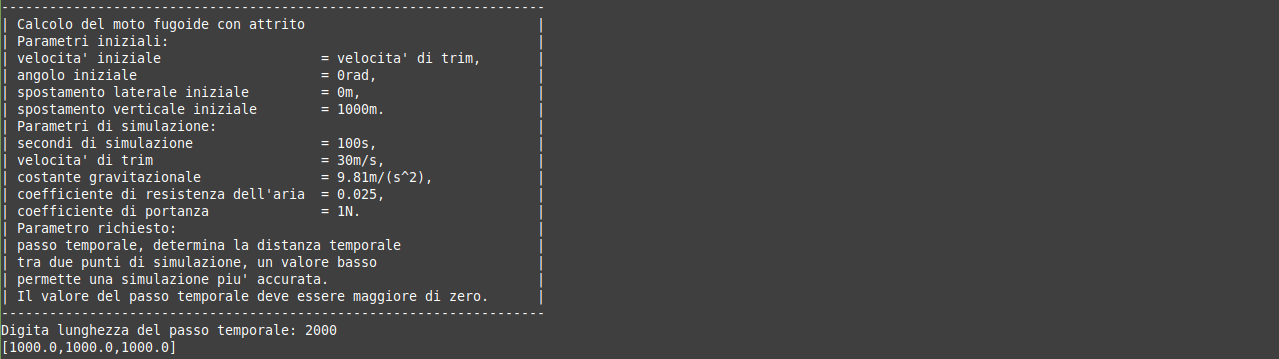
\includegraphics[width=\textwidth,height=\textheight,keepaspectratio]{05_testing/image/hs/07_test/02_misto.png}
\\
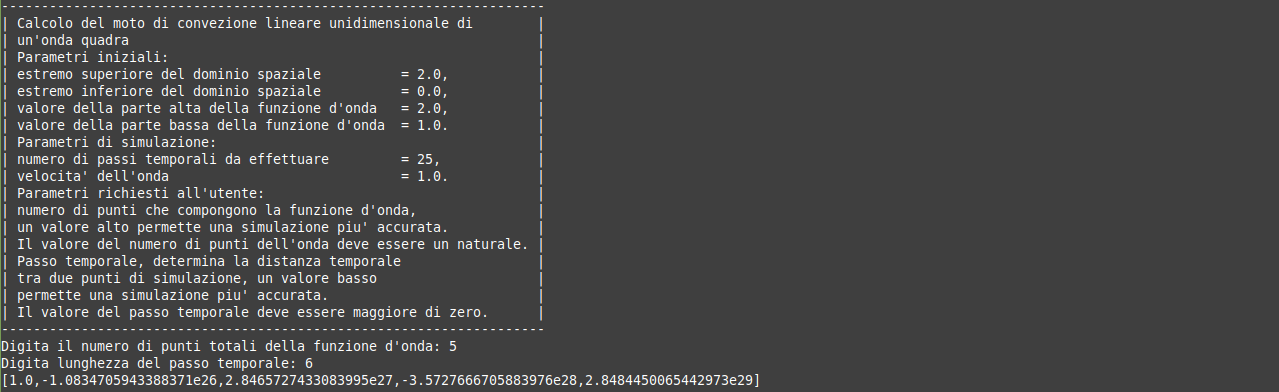
\includegraphics[width=\textwidth,height=\textheight,keepaspectratio]{05_testing/image/hs/07_test/03_misto.png}
\\
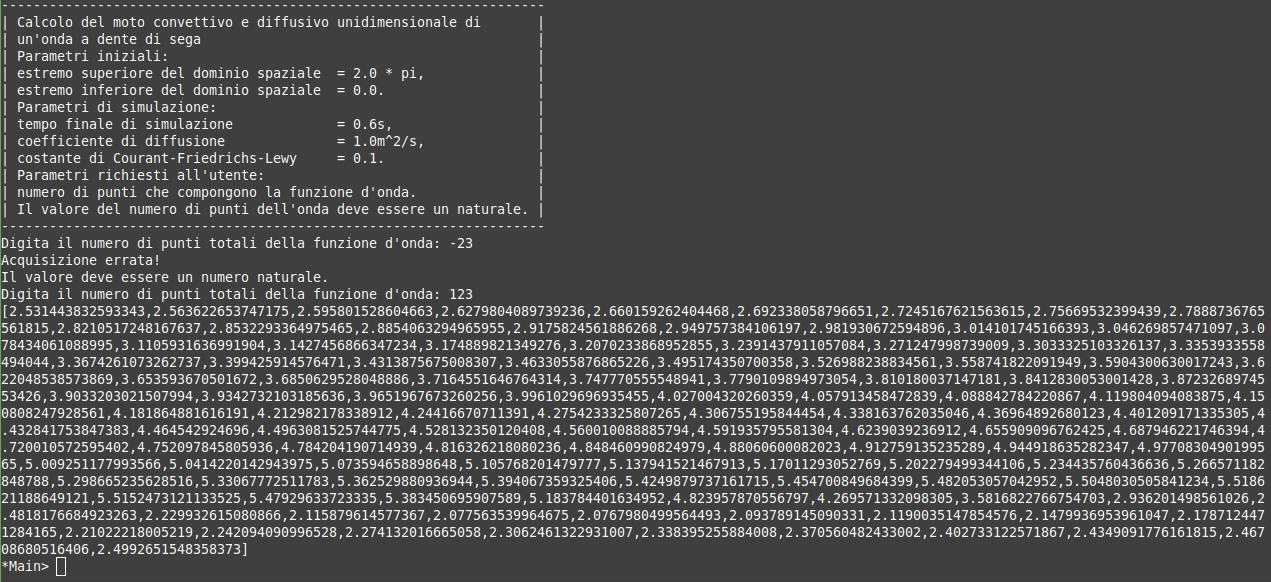
\includegraphics[width=\textwidth,height=\textheight,keepaspectratio]{05_testing/image/hs/07_test/04_misto.png}

\subsubsection*{Test 8}
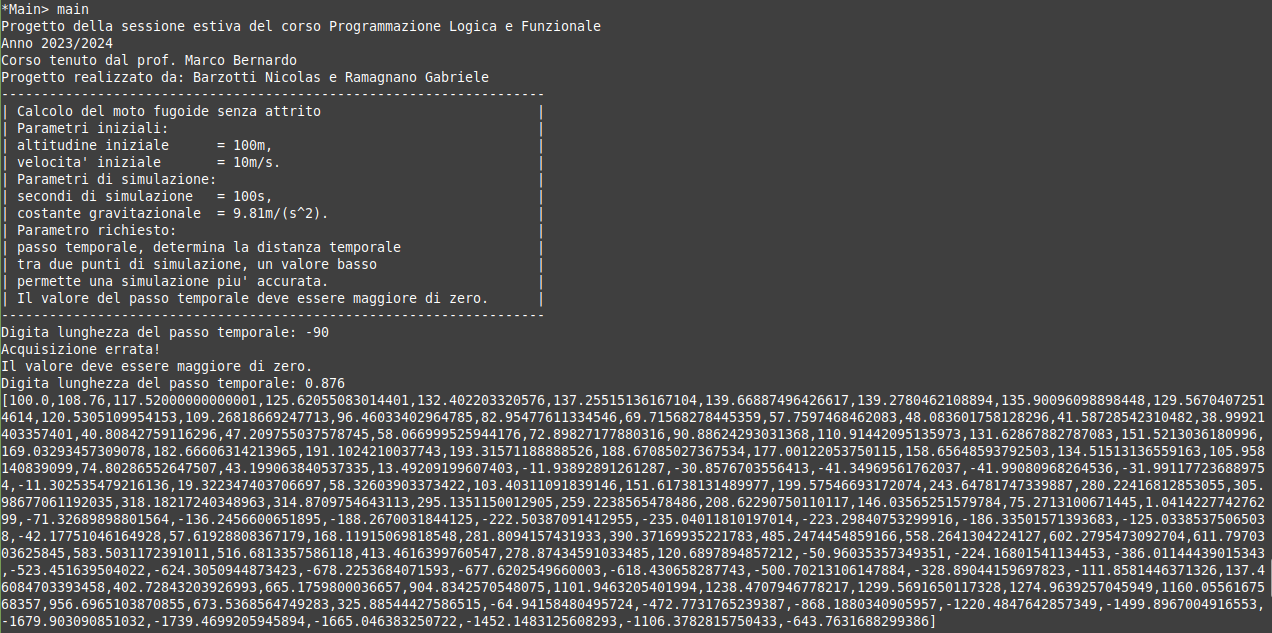
\includegraphics[width=\textwidth,height=\textheight,keepaspectratio]{05_testing/image/hs/08_test/01_misto.png}
\\
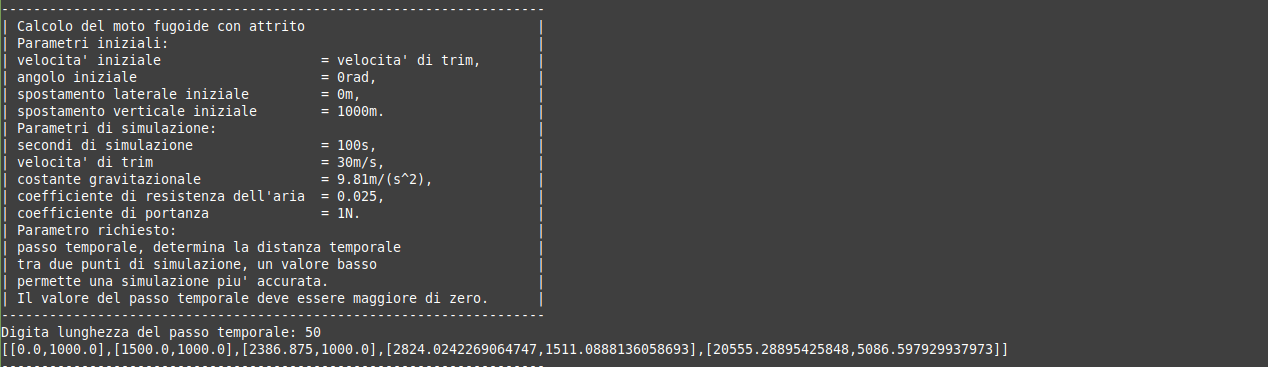
\includegraphics[width=\textwidth,height=\textheight,keepaspectratio]{05_testing/image/hs/08_test/02_misto.png}
\\
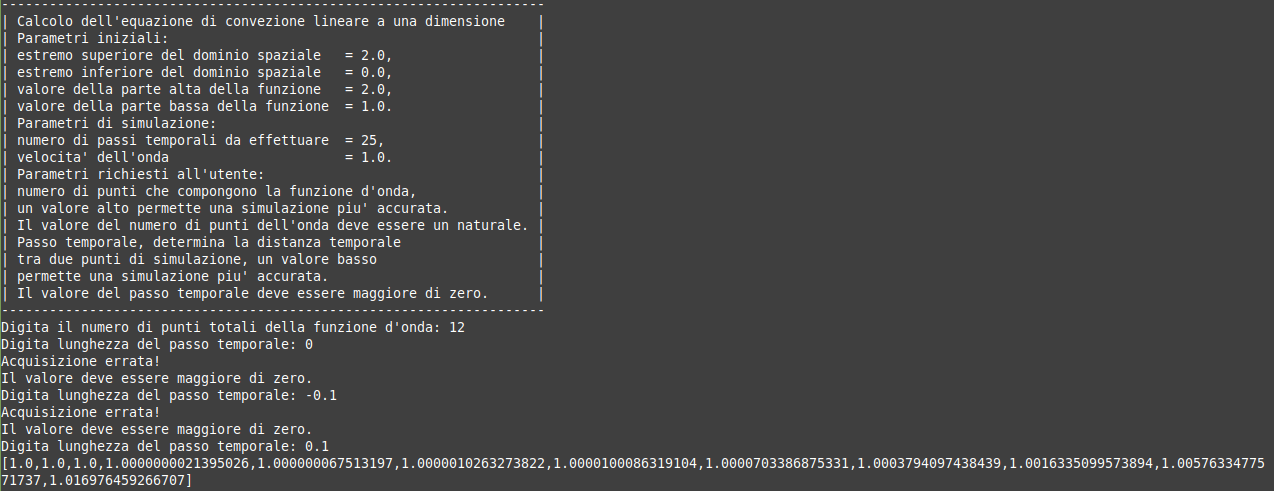
\includegraphics[width=\textwidth,height=\textheight,keepaspectratio]{05_testing/image/hs/08_test/03_misto.png}
\\
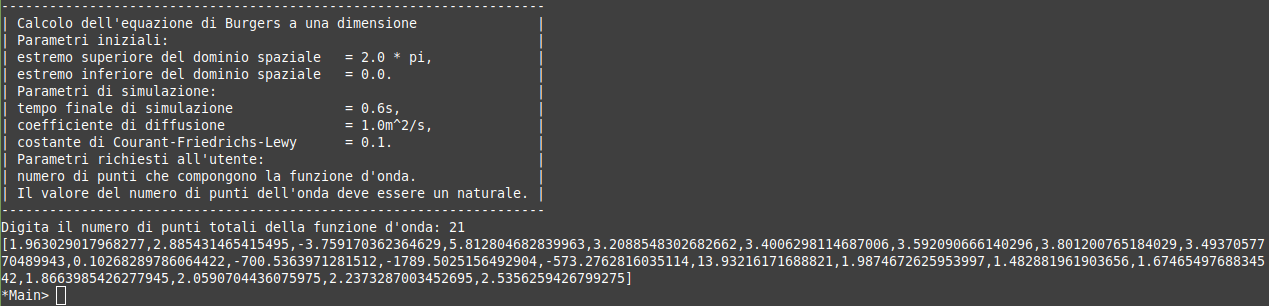
\includegraphics[width=\textwidth,height=\textheight,keepaspectratio]{05_testing/image/hs/08_test/04_misto.png}

\subsubsection*{Test 9}
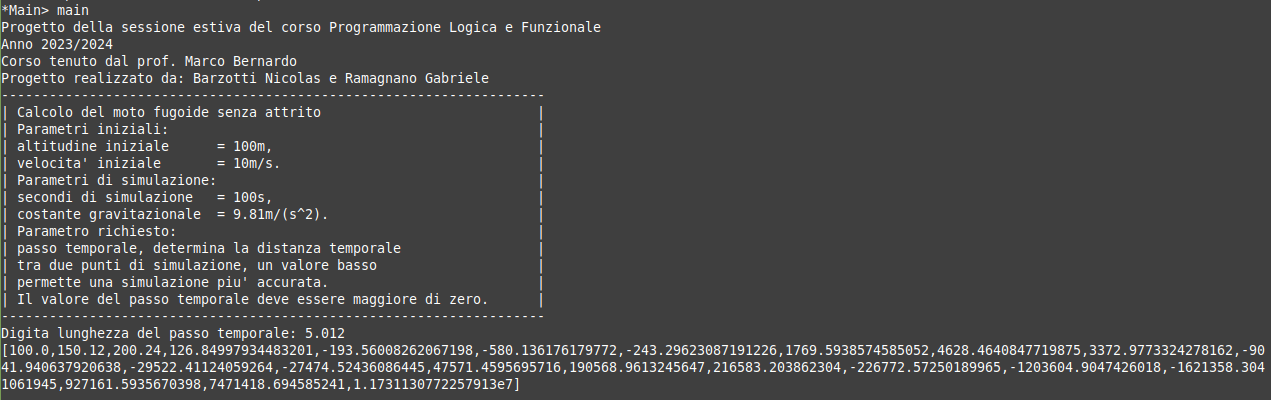
\includegraphics[width=\textwidth,height=\textheight,keepaspectratio]{05_testing/image/hs/09_test/01_misto.png}
\\
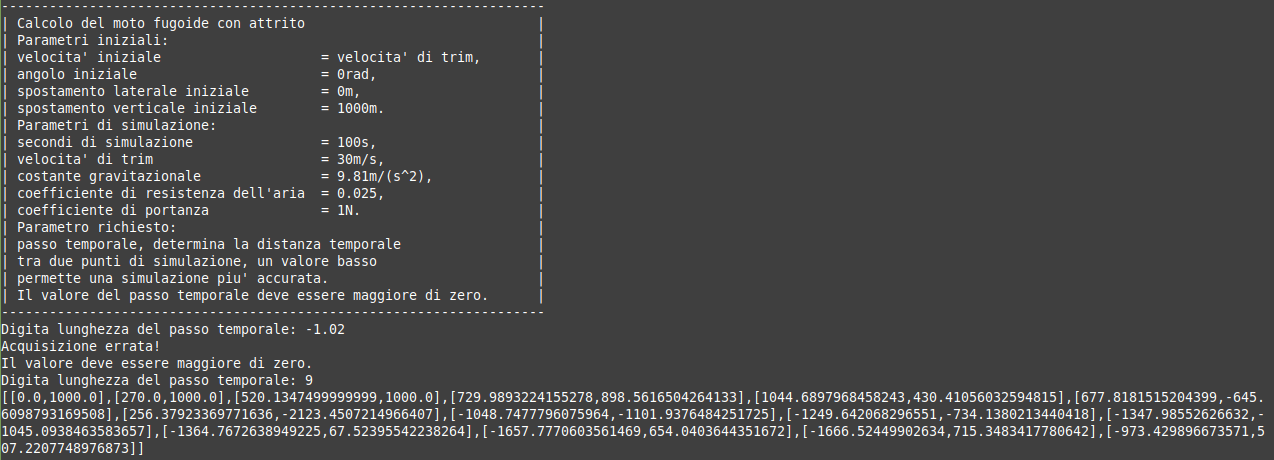
\includegraphics[width=\textwidth,height=\textheight,keepaspectratio]{05_testing/image/hs/09_test/02_misto.png}
\\
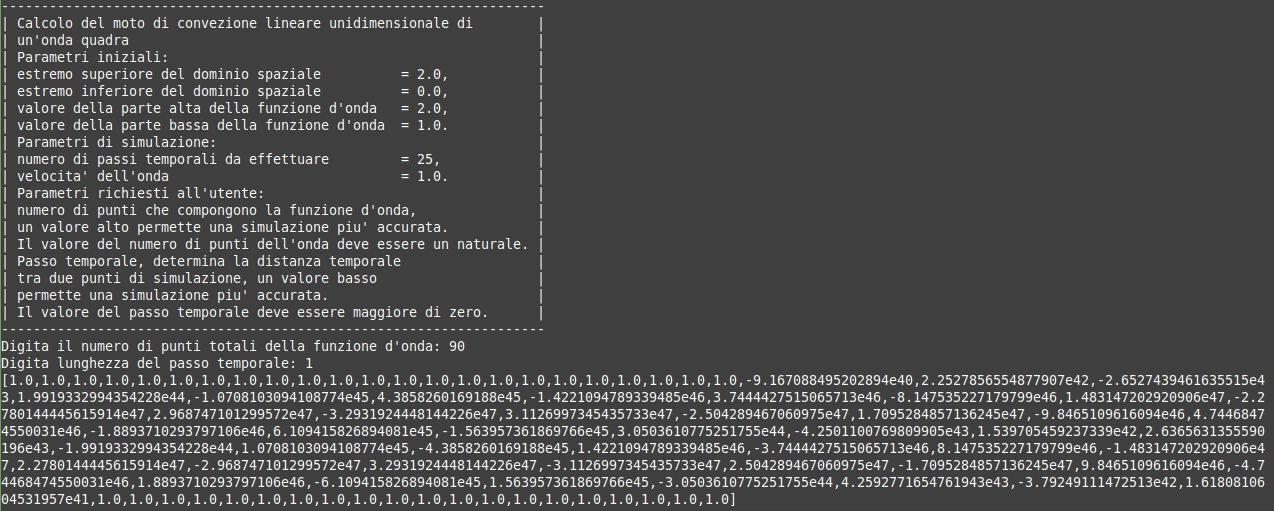
\includegraphics[width=\textwidth,height=\textheight,keepaspectratio]{05_testing/image/hs/09_test/03_misto.png}
\\
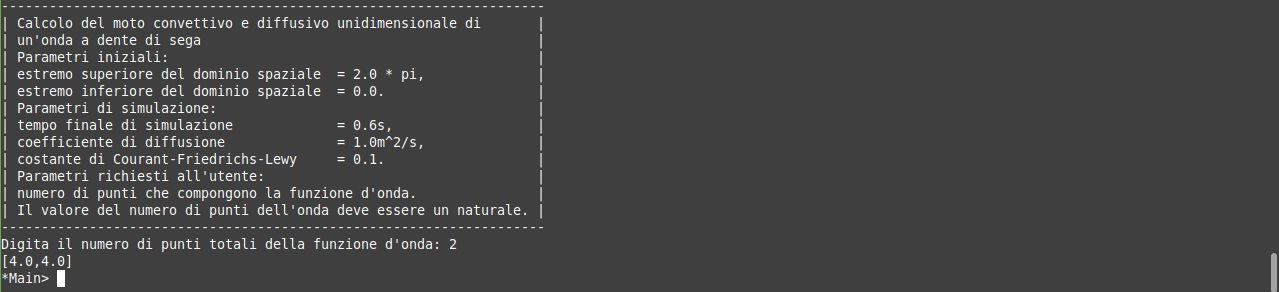
\includegraphics[width=\textwidth,height=\textheight,keepaspectratio]{05_testing/image/hs/09_test/04_misto.png}

\subsubsection*{Test 10}
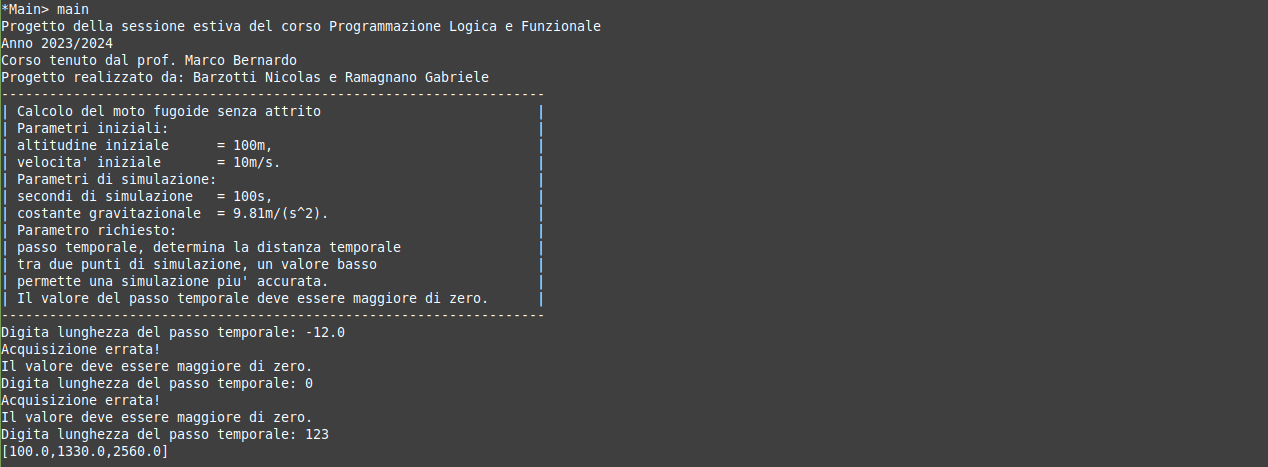
\includegraphics[width=\textwidth,height=\textheight,keepaspectratio]{05_testing/image/hs/10_test/01_misto.png}
\\
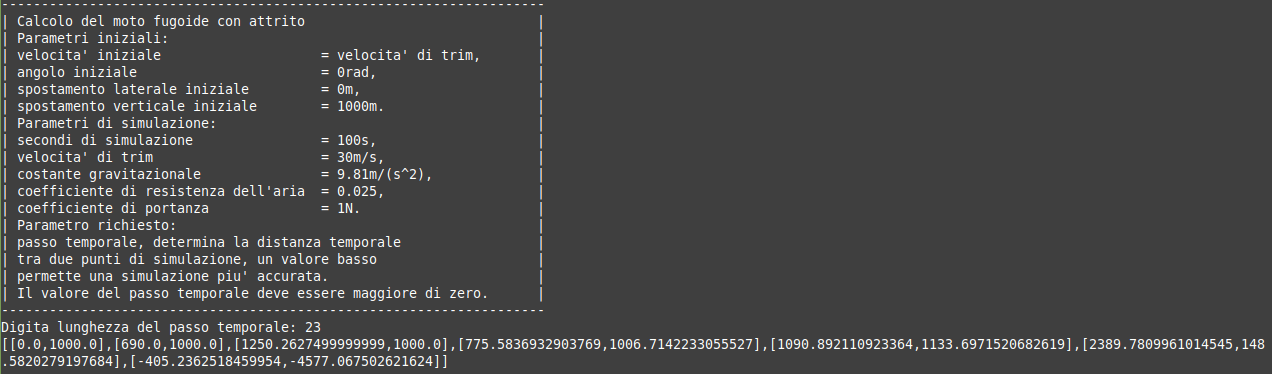
\includegraphics[width=\textwidth,height=\textheight,keepaspectratio]{05_testing/image/hs/10_test/02_misto.png}
\\
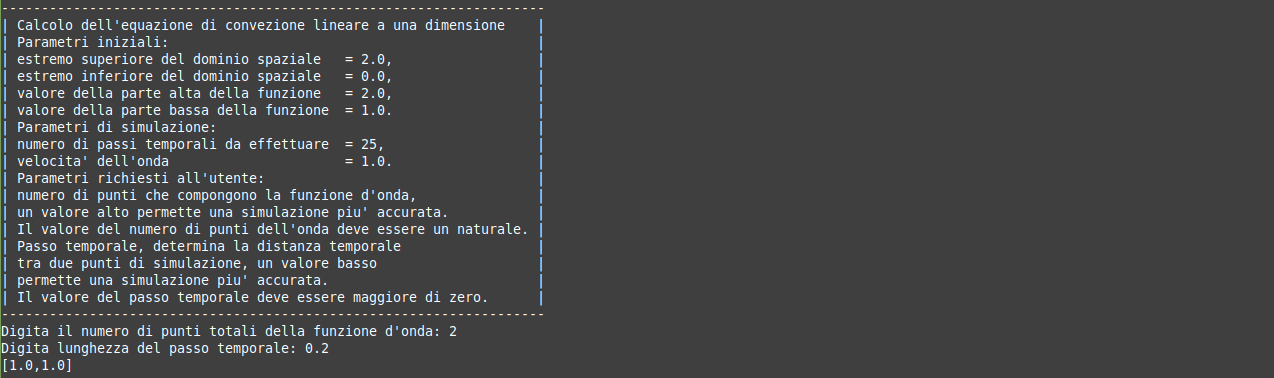
\includegraphics[width=\textwidth,height=\textheight,keepaspectratio]{05_testing/image/hs/10_test/03_misto.png}
\\
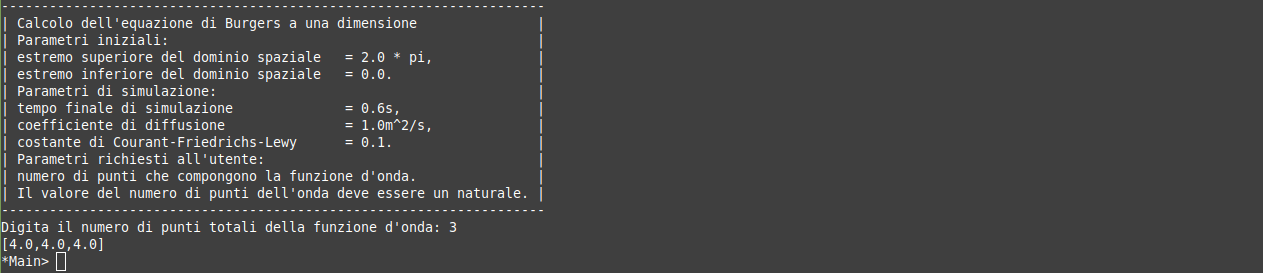
\includegraphics[width=\textwidth,height=\textheight,keepaspectratio]{05_testing/image/hs/10_test/04_misto.png}


\subsection{Prolog}

\subsubsection*{Test 1}
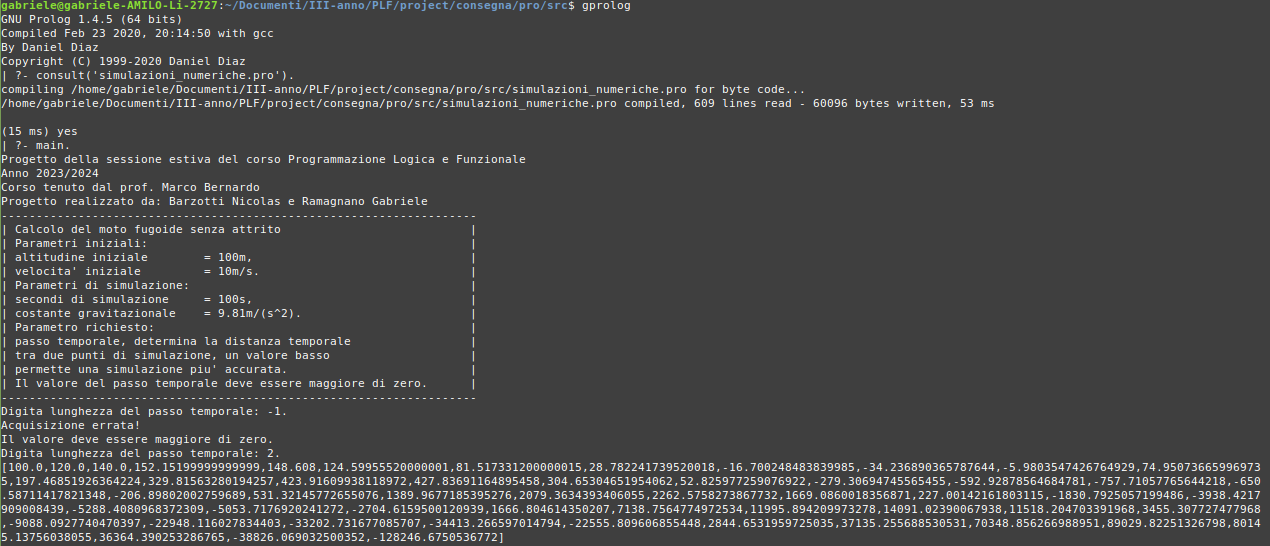
\includegraphics[width=\textwidth,height=\textheight,keepaspectratio]{05_testing/image/pro/01_test/01.png}
\\
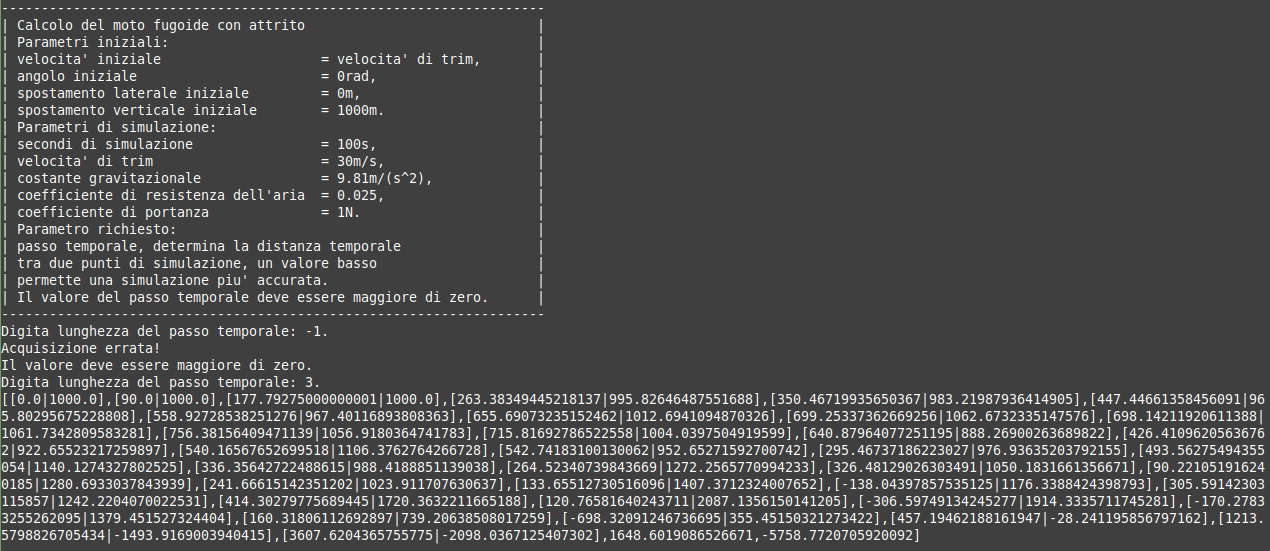
\includegraphics[width=\textwidth,height=\textheight,keepaspectratio]{05_testing/image/pro/01_test/02.png}
\\
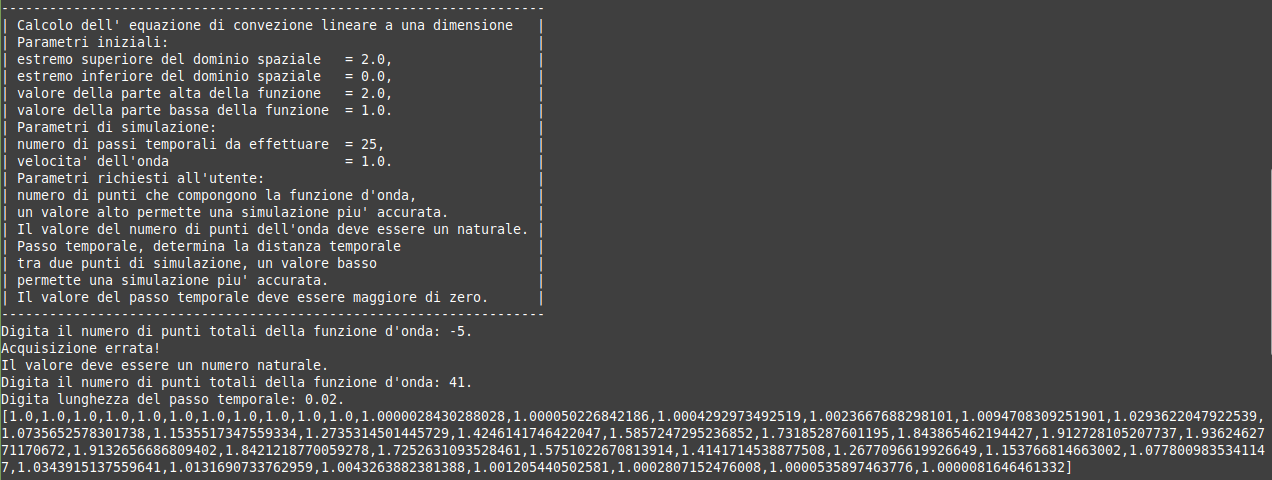
\includegraphics[width=\textwidth,height=\textheight,keepaspectratio]{05_testing/image/pro/01_test/03.png}
\\
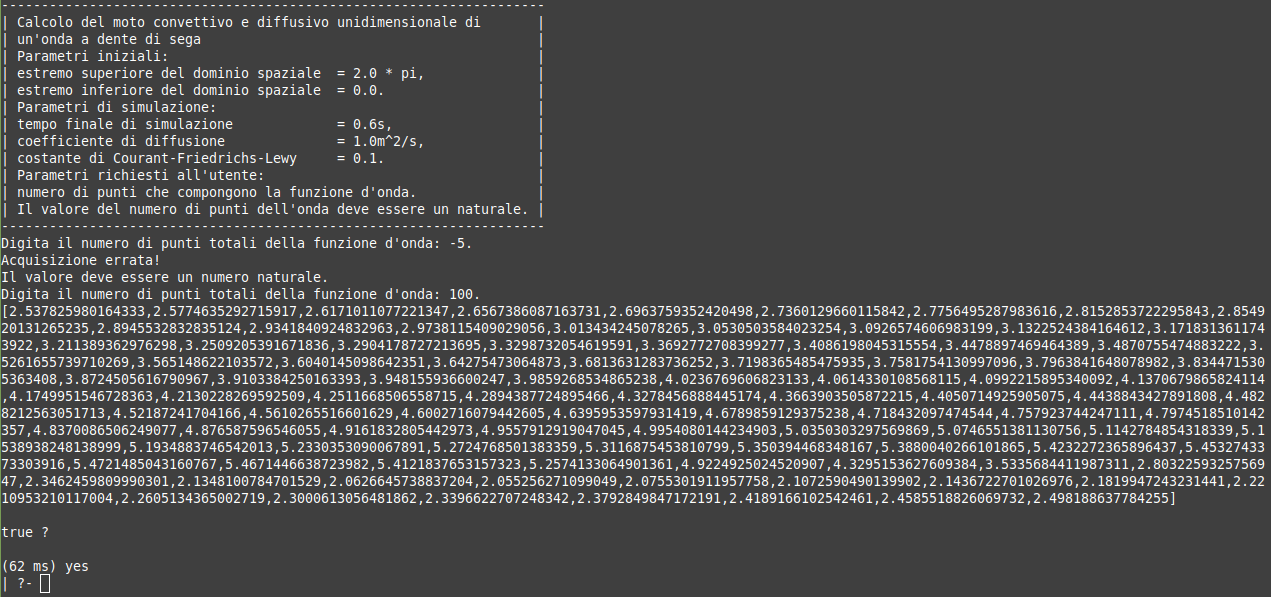
\includegraphics[width=\textwidth,height=\textheight,keepaspectratio]{05_testing/image/pro/01_test/04.png}

\subsubsection*{Test 2}
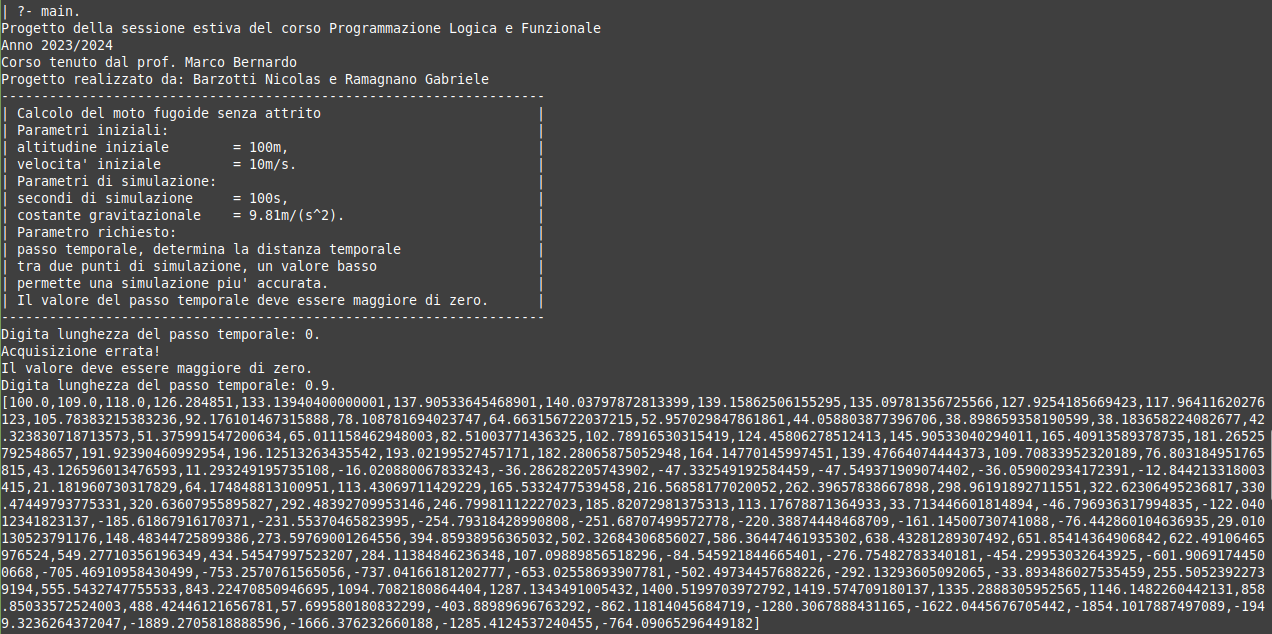
\includegraphics[width=\textwidth,height=\textheight,keepaspectratio]{05_testing/image/pro/02_test/01.png}
\\
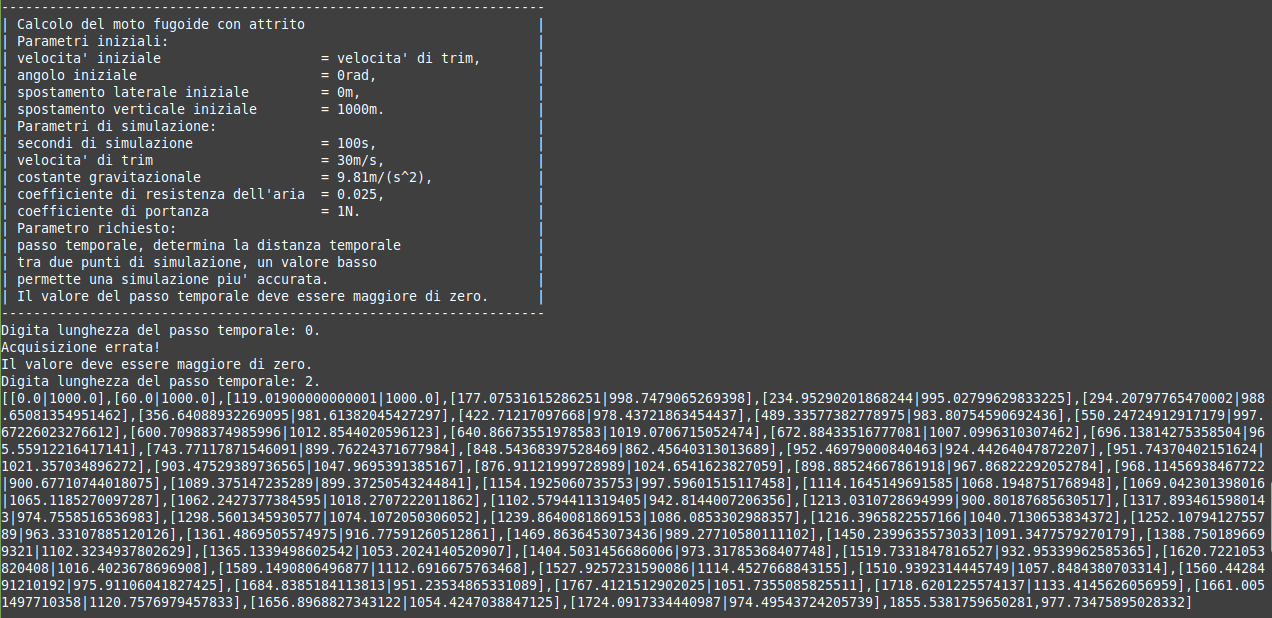
\includegraphics[width=\textwidth,height=\textheight,keepaspectratio]{05_testing/image/pro/02_test/02.png}
\\
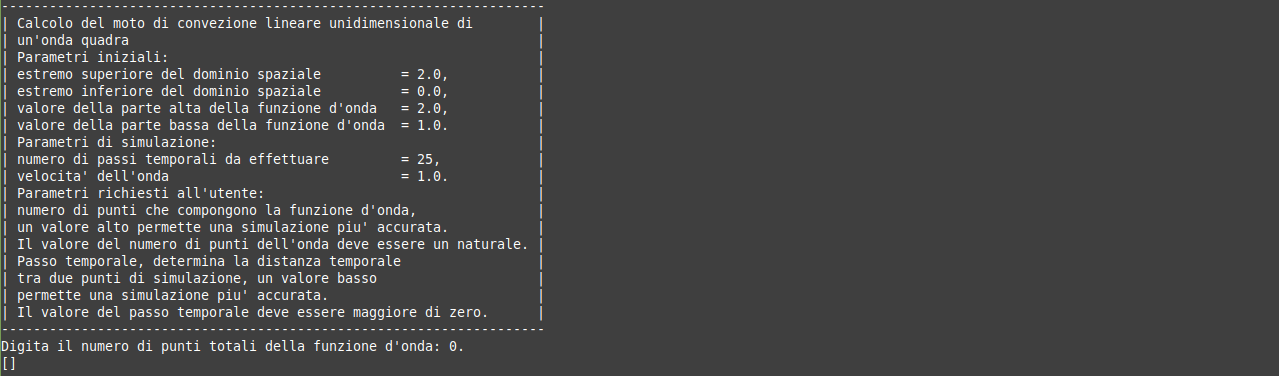
\includegraphics[width=\textwidth,height=\textheight,keepaspectratio]{05_testing/image/pro/02_test/03.png}
\\
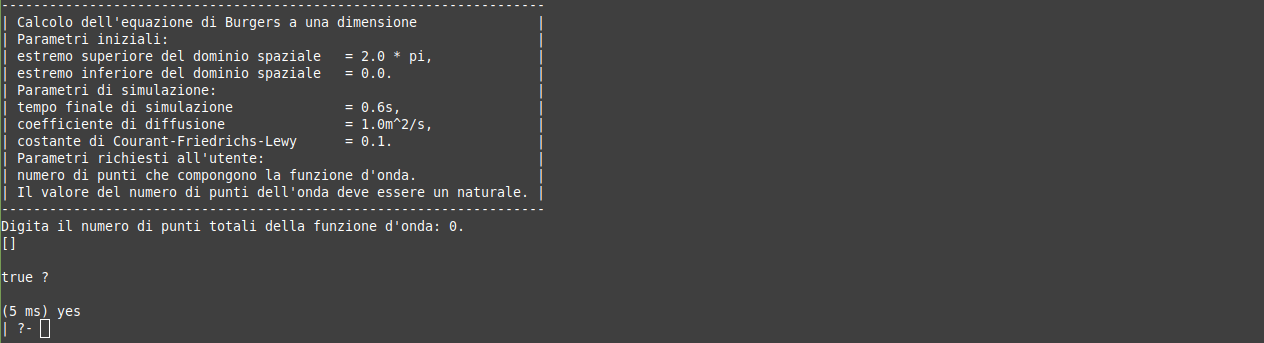
\includegraphics[width=\textwidth,height=\textheight,keepaspectratio]{05_testing/image/pro/02_test/04.png}

\subsubsection*{Test 3}
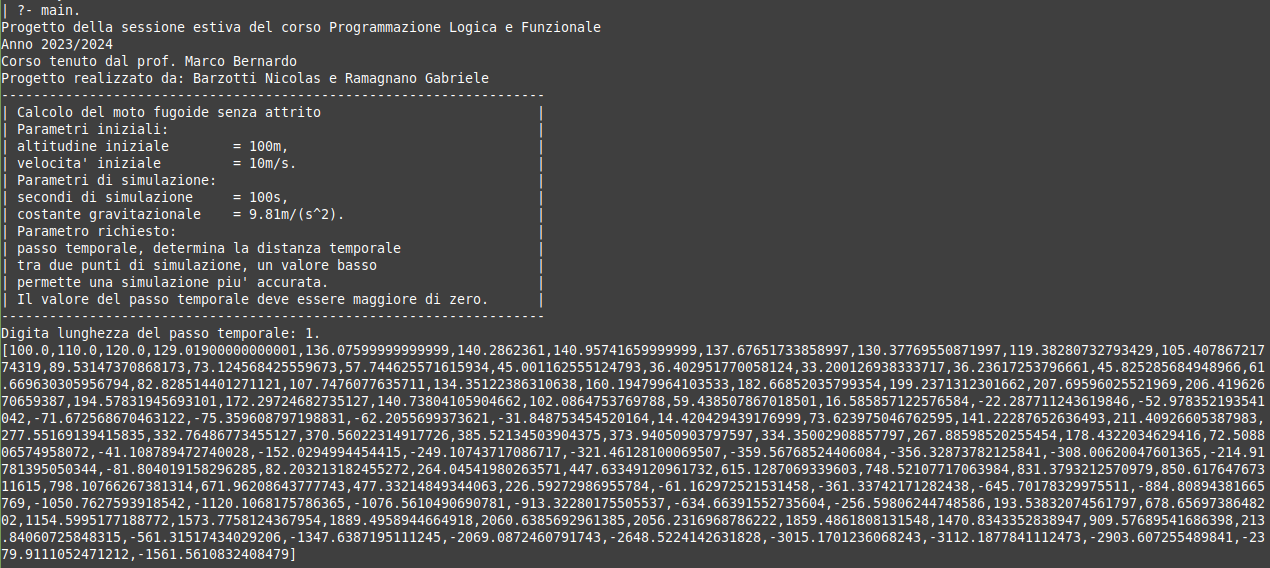
\includegraphics[width=\textwidth,height=\textheight,keepaspectratio]{05_testing/image/pro/03_test/01.png}
\\
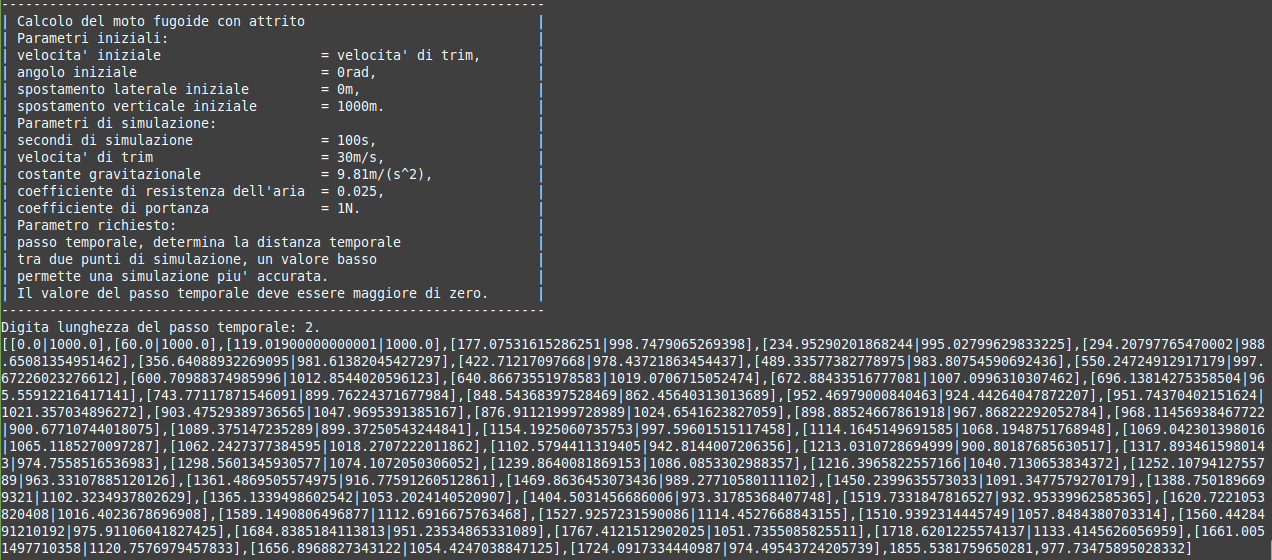
\includegraphics[width=\textwidth,height=\textheight,keepaspectratio]{05_testing/image/pro/03_test/02.png}
\\
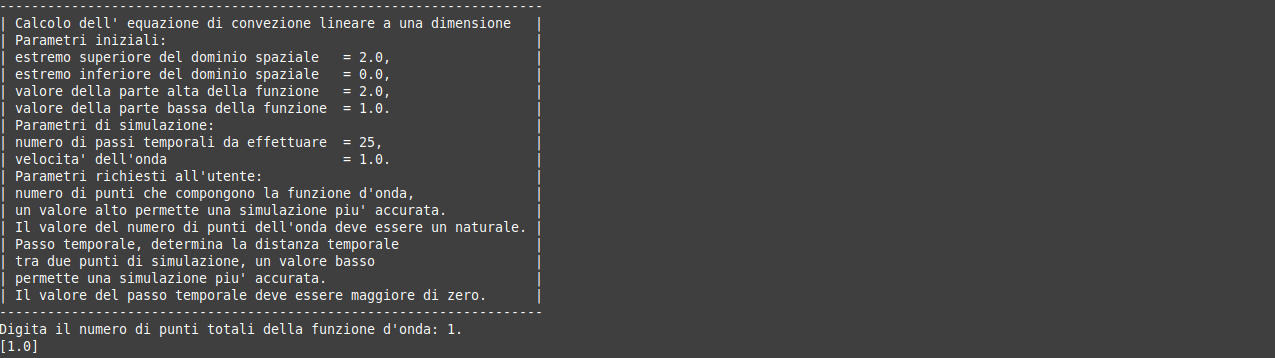
\includegraphics[width=\textwidth,height=\textheight,keepaspectratio]{05_testing/image/pro/03_test/03.png}
\\
\includegraphics[width=\textwidth,height=\textheight,keepaspectratio]{05_testing/image/pro/03_test/04.png}

\subsubsection*{Test 4}
\includegraphics[width=\textwidth,height=\textheight,keepaspectratio]{05_testing/image/pro/04_test/01.png}
\\
\includegraphics[width=\textwidth,height=\textheight,keepaspectratio]{05_testing/image/pro/04_test/02.png}
\\
\includegraphics[width=\textwidth,height=\textheight,keepaspectratio]{05_testing/image/pro/04_test/03.png}
\\
\includegraphics[width=\textwidth,height=\textheight,keepaspectratio]{05_testing/image/pro/04_test/04.png}

\subsubsection*{Test 5}
\includegraphics[width=\textwidth,height=\textheight,keepaspectratio]{05_testing/image/pro/05_test/01.png}
\\
\includegraphics[width=\textwidth,height=\textheight,keepaspectratio]{05_testing/image/pro/05_test/02.png}
\\
\includegraphics[width=\textwidth,height=\textheight,keepaspectratio]{05_testing/image/pro/05_test/03.png}
\\
\includegraphics[width=\textwidth,height=\textheight,keepaspectratio]{05_testing/image/pro/05_test/04.png}

\subsubsection*{Test 6}
\includegraphics[width=\textwidth,height=\textheight,keepaspectratio]{05_testing/image/pro/06_test/01.png}
\\
\includegraphics[width=\textwidth,height=\textheight,keepaspectratio]{05_testing/image/pro/06_test/02.png}
\\
\includegraphics[width=\textwidth,height=\textheight,keepaspectratio]{05_testing/image/pro/06_test/03.png}
\\
\includegraphics[width=\textwidth,height=\textheight,keepaspectratio]{05_testing/image/pro/06_test/04.png}

\subsubsection*{Test 7}
\includegraphics[width=\textwidth,height=\textheight,keepaspectratio]{05_testing/image/pro/07_test/01.png}
\\
\includegraphics[width=\textwidth,height=\textheight,keepaspectratio]{05_testing/image/pro/07_test/02.png}
\\
\includegraphics[width=\textwidth,height=\textheight,keepaspectratio]{05_testing/image/pro/07_test/03.png}
\\
\includegraphics[width=\textwidth,height=\textheight,keepaspectratio]{05_testing/image/pro/07_test/04.png}

\subsubsection*{Test 8}
\includegraphics[width=\textwidth,height=\textheight,keepaspectratio]{05_testing/image/pro/08_test/01.png}
\\
\includegraphics[width=\textwidth,height=\textheight,keepaspectratio]{05_testing/image/pro/08_test/02.png}
\\
\includegraphics[width=\textwidth,height=\textheight,keepaspectratio]{05_testing/image/pro/08_test/03.png}
\\
\includegraphics[width=\textwidth,height=\textheight,keepaspectratio]{05_testing/image/pro/08_test/04.png}

\subsubsection*{Test 9}
\includegraphics[width=\textwidth,height=\textheight,keepaspectratio]{05_testing/image/pro/09_test/01.png}
\\
\includegraphics[width=\textwidth,height=\textheight,keepaspectratio]{05_testing/image/pro/09_test/02.png}
\\
\includegraphics[width=\textwidth,height=\textheight,keepaspectratio]{05_testing/image/pro/09_test/03.png}
\\
\includegraphics[width=\textwidth,height=\textheight,keepaspectratio]{05_testing/image/pro/09_test/04.png}

\subsubsection*{Test 10}
\includegraphics[width=\textwidth,height=\textheight,keepaspectratio]{05_testing/image/pro/10_test/01.png}
\\
\includegraphics[width=\textwidth,height=\textheight,keepaspectratio]{05_testing/image/pro/10_test/02.png}
\\
\includegraphics[width=\textwidth,height=\textheight,keepaspectratio]{05_testing/image/pro/10_test/03.png}
\\
\includegraphics[width=\textwidth,height=\textheight,keepaspectratio]{05_testing/image/pro/10_test/04.png}



\end{document}
